\documentclass[pdf]{beamer}
\mode<presentation>{}

\usetheme{Frankfurt}
\usepackage{listings}
\usepackage{color}
\usepackage{amsmath}
\usepackage{wasysym}
\usepackage{bm}

\usefonttheme[onlymath]{serif}

\newcommand\norm[1]{\left\lVert#1\right\rVert}


%=== Adding page numbers
\addtobeamertemplate{navigation symbols}{}{%
    \usebeamerfont{footline}%
    \usebeamercolor[fg]{footline}%
    \hspace{1em}%
    \insertframenumber/\inserttotalframenumber
}
\setbeamercolor{footline}{fg=blue}
\setbeamerfont{footline}{series=\bfseries}
%===

%% preamble
\title[Intro to Deep Learning]{A Very Brief Introduction to Neural Networks and Deep Learning}

\author{Ashley Lee, Isabel Restrepo, \& Paul Stey}
\date{\today}




\begin{document}

%% title frame
\begin{frame}
\titlepage
\end{frame}



\begin{frame}<beamer>{Table of Contents}
	\tableofcontents[currentsection, 
				 currentsubsection, 
				 sectionstyle=show, 
				 subsectionstyle=show]
\end{frame}

\section{Background}

\subsection{Neural Network Basics}
	\begin{frame}{What is a neural network?}
		\begin{enumerate}
			\item A species of directed acyclic graphs (usually)
			\item ``Universal function approximator''
			\item ``An engineering solution to a statistics problem''
		\end{enumerate}
	\end{frame}

	\begin{frame}{What do neural networks do?}
	Like many other statistical or machine learning models (e.g., GLM, random forests, boosting), neural networks:
	
	\vspace{1em}
	
		\begin{enumerate}
			\item Attempt to approximate a data-generating mechanism
			\item Can be used for classification problems
			\item Can be used for regression problems
			\item Can also be used for dimension reduction like principal components analysis (PCA)
 
		\end{enumerate}
	\end{frame}

\subsection{History}
	\begin{frame}{History of Neural Networks}
	The history of neural networks is long and tumultuous.
	\vspace{2em}
		\begin{enumerate}
			\item McCulloch and Pitts (1943) ``\textit{A Logical Calculus of Ideas Immanent in Nervous Activity}''
			\item Rosenblatt (1958) ``\textit{The Perceptron: A Probabilistic Model For Information Storage And Organization In The Brain}''
		\end{enumerate}
	\begin{center}
		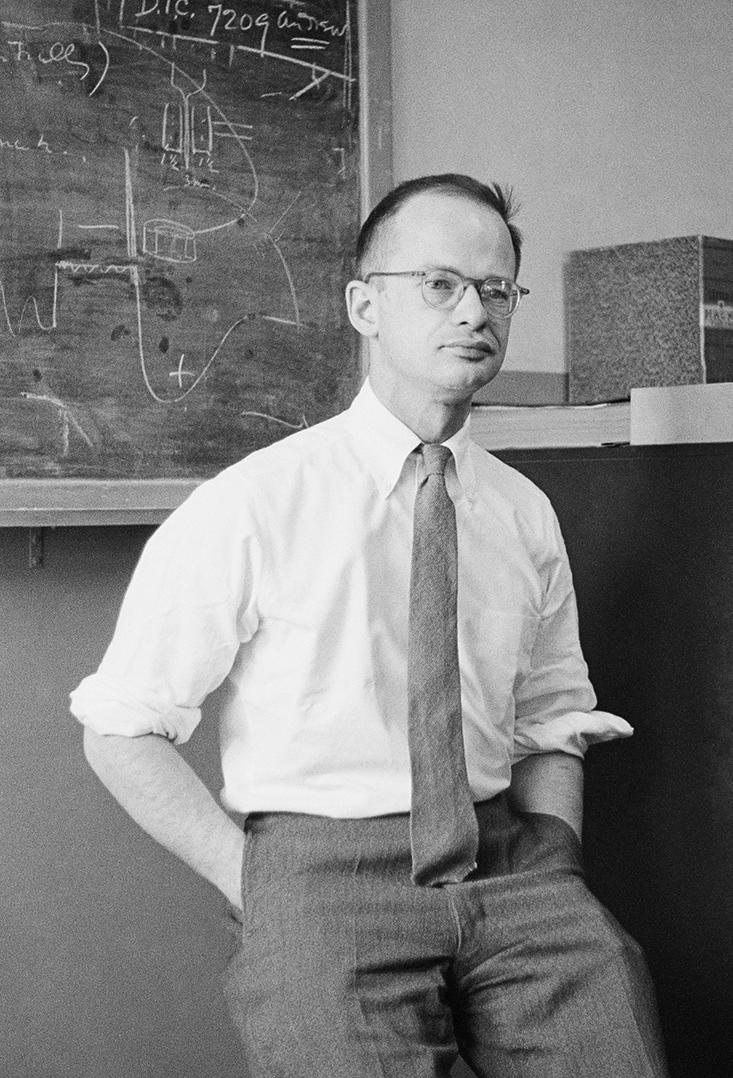
\includegraphics[scale=0.08]{/Users/pstey/projects_code/deep_learning_group/slides/intro_deep_learning/images/pitts.jpg}
		\hspace{3em}
		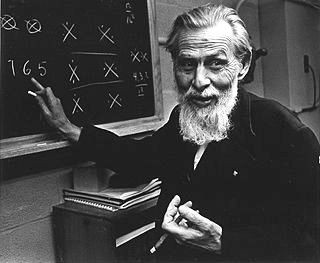
\includegraphics[scale=0.25]{/Users/pstey/projects_code/deep_learning_group/slides/intro_deep_learning/images/mcculloch.jpeg}
	\end{center}
	\end{frame}
	
	\begin{frame}{More Recently}
	Neural networks are experiencing a major resurgence. There are at least two reasons.
	
		\begin{enumerate}
			\item Better algorithms for back-propagation
			\item GPUs are well suited to building neural networks
				\begin{itemize}
					\item Matrix multiplies can be made embarrassingly parallel 
					\item GPUs have much better memory bandwidth
				\end{itemize}
			\item More labeled data
		\end{enumerate}
	\end{frame}



\subsection{Mechanics of Neural Networks}
	\begin{frame}{The Multilayer Perceptron}
	\begin{center}
		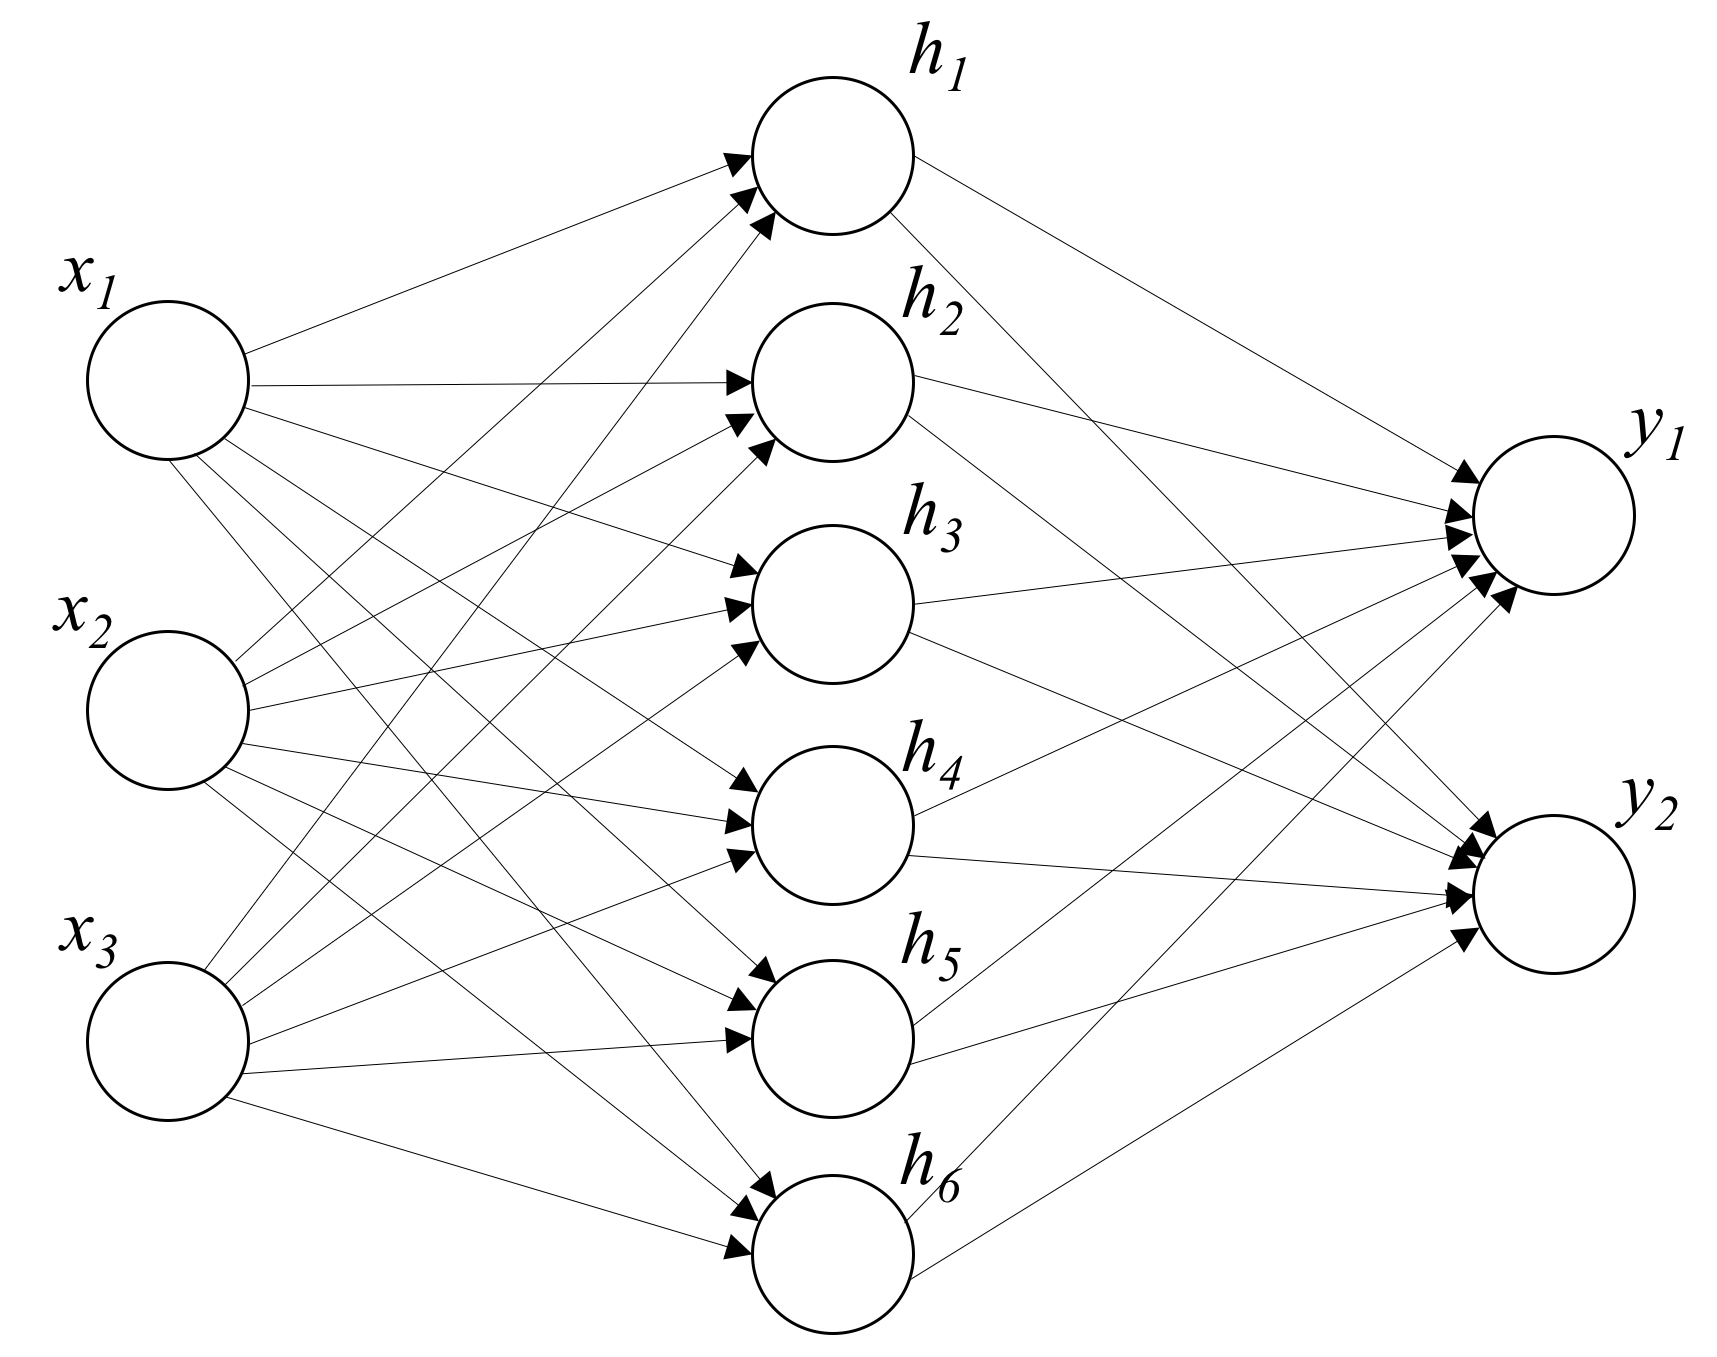
\includegraphics[scale=0.15]{/Users/pstey/projects_code/deep_learning_group/slides/intro_deep_learning/images/neural_network2.png}
	\end{center}
	\end{frame}

	\begin{frame}{Single Neuron}
	\begin{columns}
		\begin{column}{0.5\textwidth}
		A single neuron takes inputs, $x_j$, and applies the weights, $w_{\cdot j}$ to the input by computing the dot product of the vectors $x$ and $w$. The result is the input to the ``activation'' function.

		\end{column}
	
		\begin{column}{0.5\textwidth}
		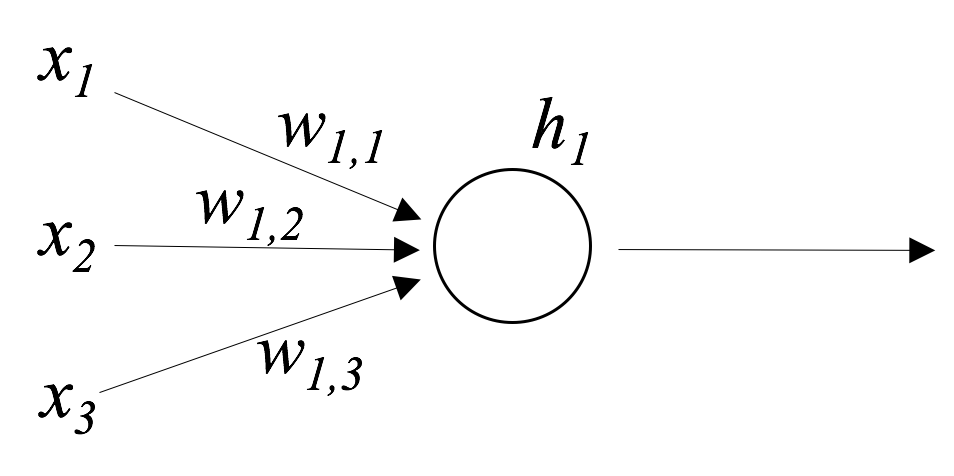
\includegraphics[scale=0.15]{/Users/pstey/projects_code/deep_learning_group/slides/intro_deep_learning/images/neuron2.png}
		\end{column}
	\end{columns}
	\end{frame}

	\begin{frame}{Activation Functions}
	
	The notion of an activation function comes again from the theoretical relationship to neurons in the brain.
	\vspace{2em}
	
	Activation functions are analogous to ``link'' functions in generalized linear models (GLMs). 
	
	\vspace{2em} 
	In fact, one common activation function is the sigmoid function, which is just our old friend the logistic function which you are using when you fit logistic regression models.
	\end{frame}
	
	
	\begin{frame}{Purpose of Activation Functions}
	
	There are a few reasons we use activation functions.	
	\vspace{2em}
	
	The most basic reason is that---like link functions in GLMs---we want to take some linear predictor and transform it so that it is bounded appropriate. For instance, the value of logistic function is in the range $(0, 1)$. 
	
	\vspace{2em}
	
	And the second key reason is that this allows us to introduce non-linearities. Recall that a neural network (like many statistical or machine learning models) is trying to approximate a data-generating mechanism. So we are trying to approximate a function that might be very complex and include many non-linearities.
	\end{frame}
	
	
	\begin{frame}{Common Activation Functions}
	\begin{columns}
	\begin{column}{0.5\textwidth}
	Some common activation functions include the following: 
	\vspace{1em}
	\begin{enumerate}
		\item Sigmoid (i.e., logistic)
		\item Hyperbolic tangent: $tanh$
		\item Rectified linear unit (ReLU)
		\item softplus
	\end{enumerate}
	\end{column}
	
	\begin{column}{0.5\textwidth}
	\begin{center}
		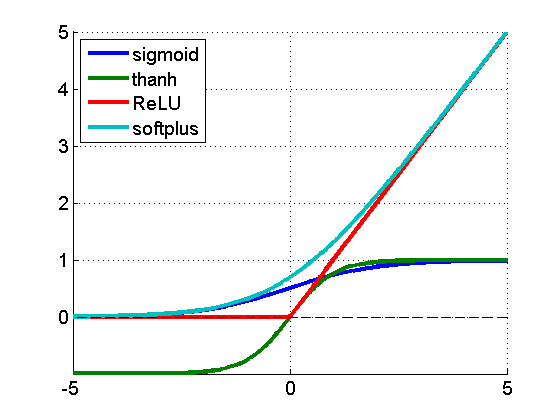
\includegraphics[scale=0.35]{/Users/pstey/projects_code/deep_learning_group/slides/intro_deep_learning/images/activation_functions.png}
	\end{center}
	\end{column}
	\end{columns}
	\end{frame}

	\begin{frame}{Sigmoid Functions}
	\begin{columns}
	\begin{column}{0.5\textwidth}
	Sigmoid function: $\phi(z) = \frac{1}{1 + e^{-z}}$
	\vspace{1em}
	\begin{enumerate}
		\item Range between 0 and 1
		\item Sometimes interpreted as probability
		\item Special case of the softmax: $\psi(z)_j = \frac{e^{z_j}}{\sum_{k = 1}^K e^{z_k}}$, which is used for vector-value outcome
	\end{enumerate}
	\end{column}
	
	\begin{column}{0.5\textwidth}
	\begin{center}
		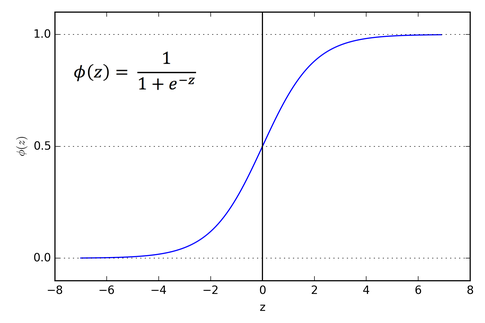
\includegraphics[scale=0.35]{/Users/pstey/projects_code/deep_learning_group/slides/intro_deep_learning/images/sigmoid_activation.png}
	\end{center}
	\end{column}
	\end{columns}
	\end{frame}



	\begin{frame}{Rectified Linear Unit (ReLU)}
	\begin{columns}
	\begin{column}{0.5\textwidth}
	ReLU: $f(z) = max(0, z)$
	\vspace{1em}
	\begin{enumerate}
		\item Range between 0 and $\inf$
		\item Biological justification	
	\end{enumerate}
	\end{column}
	
	\begin{column}{0.5\textwidth}
	\begin{center}
		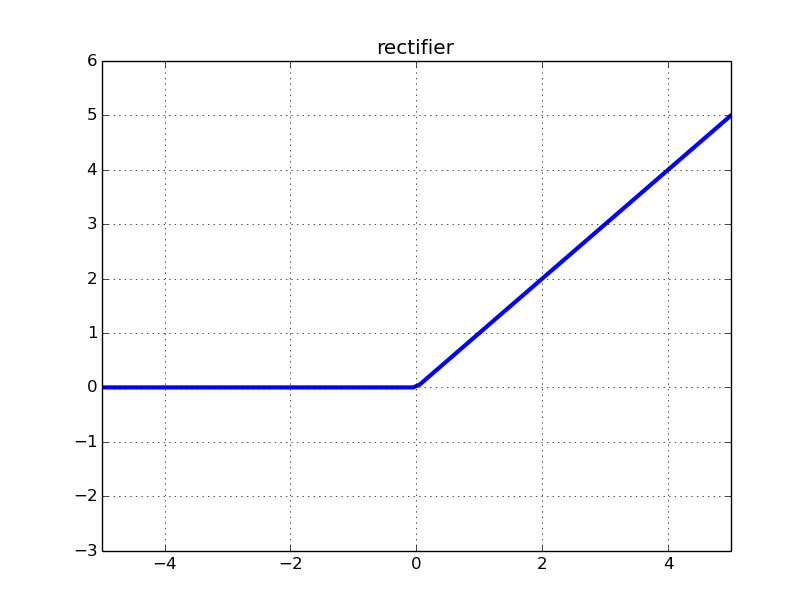
\includegraphics[scale=0.30]{/Users/pstey/projects_code/deep_learning_group/slides/intro_deep_learning/images/relu_activation.png}
	\end{center}
	\end{column}
	\end{columns}
	\end{frame}

	
	\begin{frame}{Activation Functions}
	For the hidden layers of neural networks, ReLUs---or some variation thereof---tend to be the most common.
	
	\vspace{2em}
	
	Sigmoid (and probably $tanh$) are not frequently used in the hidden layers more because of the vanishing gradient problem (discussed later).
	\end{frame}



\section{CNNs}
	\subsection{Convolutional Neural Network (CNNs)}
	\begin{frame}{Convolutional Neural Networks}
	\begin{columns}
	\begin{column}{0.5\textwidth}
	\vspace{3em}
	
	Why do we need ConvNets?
	\end{column}

	\begin{column}{0.5\textwidth}
	\begin{center}
		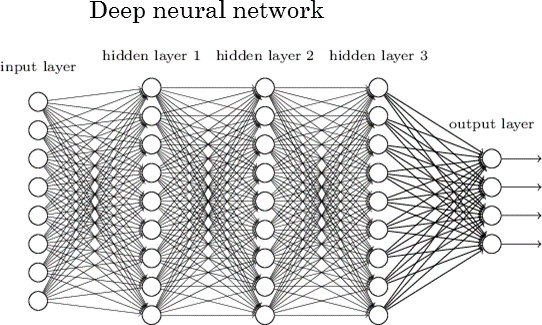
\includegraphics[scale=0.3]{/Users/pstey/projects_code/deep_learning_group/slides/intro_deep_learning/images/large_neural_net.png}
		
	\end{center}
	
	\end{column}
	\end{columns}
	
	\begin{enumerate}
		\item Regular neural nets don't scale well to images
			\begin{itemize}
				\item For images of size $32 \times 32 \times 3$, a \textit{single} fully-connected neuron in the first layer would have $3072$ weights.
				\item Images of size $200 \times 200 \times 3$, a \textit{single} gives $120000$ weights.

			\end{itemize}
		\item Full connectivity is wasteful and the huge number of parameters would quickly lead to overfitting.
		
	\end{enumerate}
	\end{frame}




	\begin{frame}{CNNs}
	What are ConvNets?
	\vspace{1em}
	
	\begin{enumerate}
		\item ConvNets are very similar to neural networks discussed thus far. Dot product, followed by non-linearity, and loss function at the end.
		\item Explicit assumption that input are images.
		\item Layers have neurons arranged in 3 dimensions (width, height, depth) to form an \textbf{activation volume}
	\end{enumerate}
	
	\begin{center}
	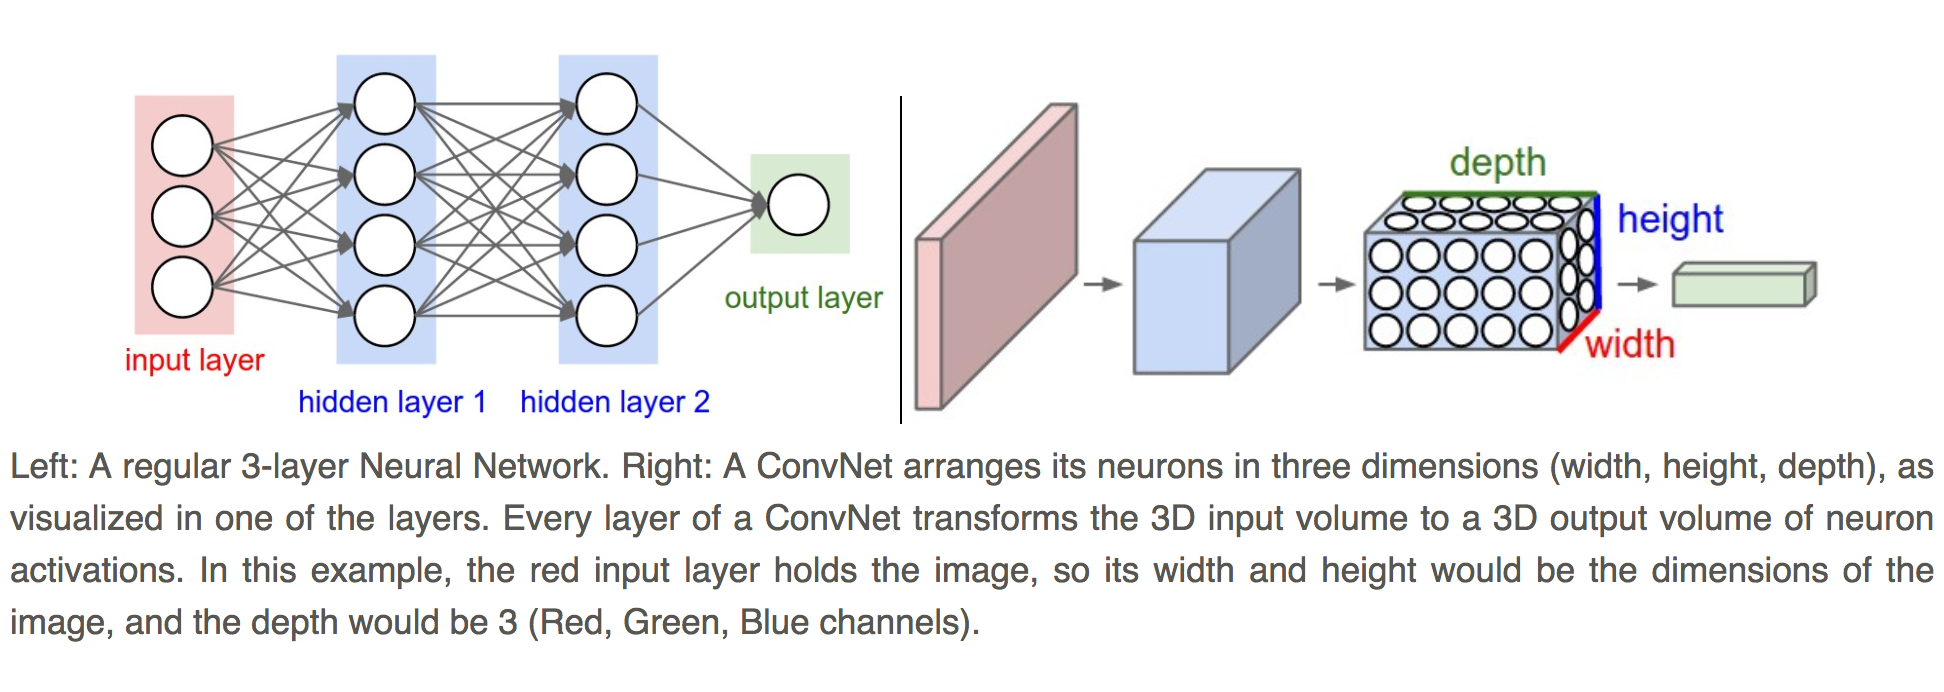
\includegraphics[scale=0.15]{/Users/pstey/projects_code/deep_learning_group/slides/intro_deep_learning/images/cnn.png}
	
	\end{center}
	\end{frame}


	\begin{frame}{CNN Architecture}
	Types of layers used to build ConvNets
	
	\vspace{1em}
	
	\begin{enumerate}
		\item Convolutional Layer
			\begin{itemize}
				\item Input: 3-d volume
				\item Output: 3-d volume
				\item Convolve ``filters'' with small regions in the image
				\item Output depth, depends on the number of filters
			\end{itemize}
		\item Pooling Layer
			\begin{itemize}
				\item Downsampling along spatial dimensions (width, height)
			\end{itemize}
		\item Fully-Connected Layer (what we've seen so far)
			\begin{itemize}
				\item Compute class score. Dimensions are transformed to $1 \times 1 \times k$, where $k$ is number of classes 
			\end{itemize}
		
	\end{enumerate}
	\end{frame}	


	\begin{frame}{CNN Architecture}
	\begin{center}
		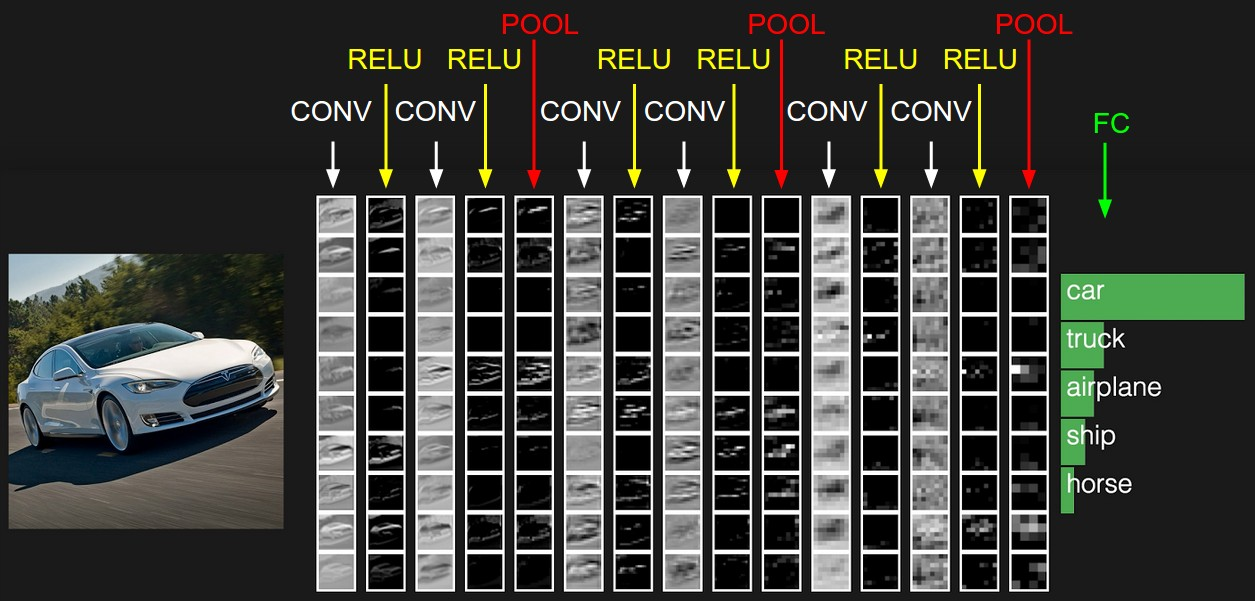
\includegraphics[scale=0.21]{/Users/pstey/projects_code/deep_learning_group/slides/intro_deep_learning/images/convnet.jpeg}
	\end{center}

	\vspace{1em}
	
	\begin{enumerate}
		\item CONV/FC layers perform transformations that are a function of not only the activations in the input volume, but also of the parameters (weights and biases of neurons).
		\item RELU/POOL layers will implement a fixed function (e.g., ReLU $= max(0, x)$)
	\end{enumerate}
	\end{frame}

	\begin{frame}{Classical Computer Vision}
	\begin{center}
		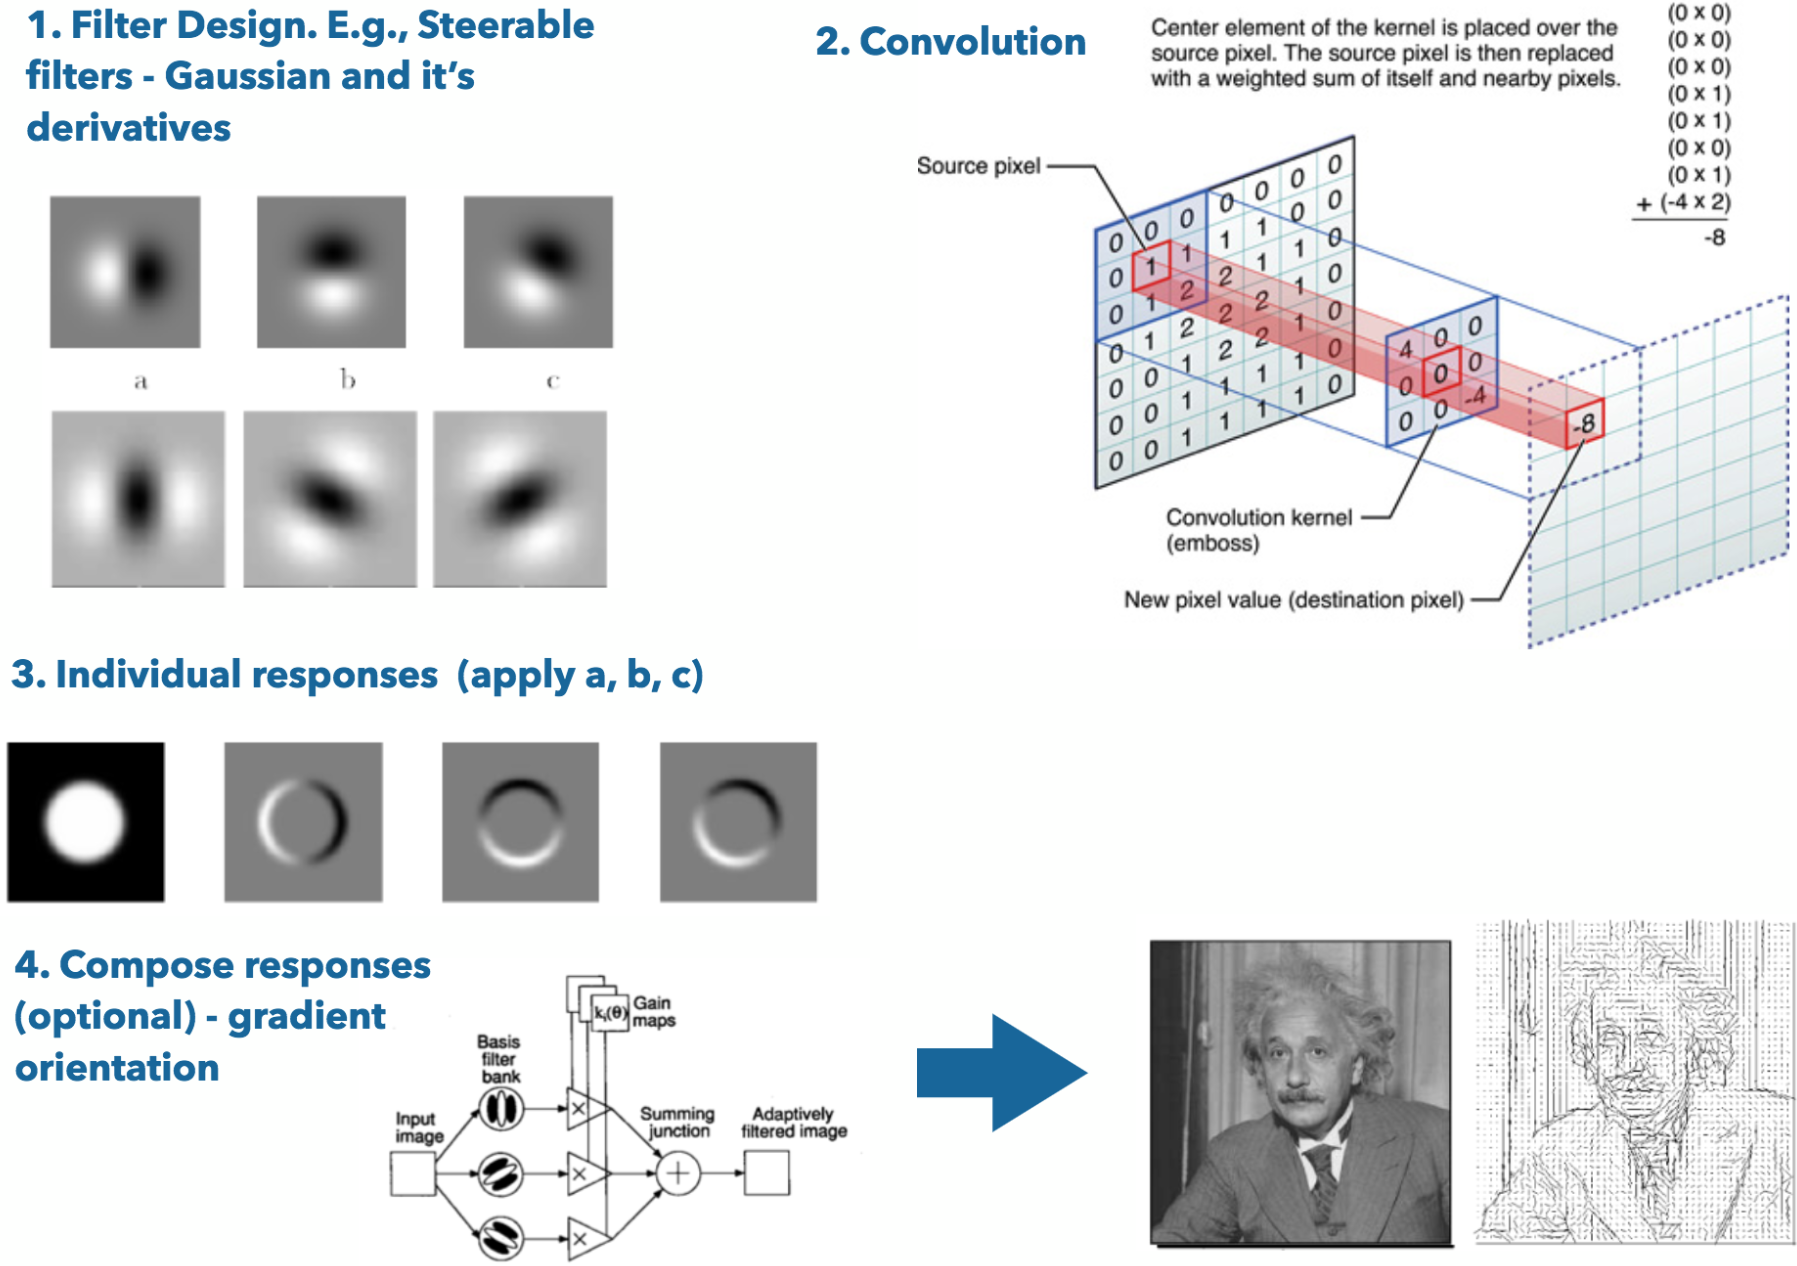
\includegraphics[scale=0.16]{/Users/pstey/projects_code/deep_learning_group/slides/intro_deep_learning/images/classic_compvision.png}
	\end{center}
	\end{frame}

	\begin{frame}{Convolutional Layer - Local Connectivity}
	Connecting each Neuron to the Input Volume
	\vspace{1em}
	\begin{enumerate}
		\item \textbf{Receptive Field (hyper-parameter):} Spatial extend of each neuron = filter size
		\item Connections are local in space (along width and height), but always full along the entire depth of the input volume.
			\vspace{1em}
			\begin{itemize}
				\item Example: Suppose an input volume had size $16 \times 16 \times 20$. Then using an example receptive field size $3 \times 3 \times 20 = 180$ connections to the input volume. Notice that, again, the connectivity is local in space (i.e., $3 \times 3$), but full along the input depth (20)
			\end{itemize}
	\end{enumerate}
	\begin{center}
		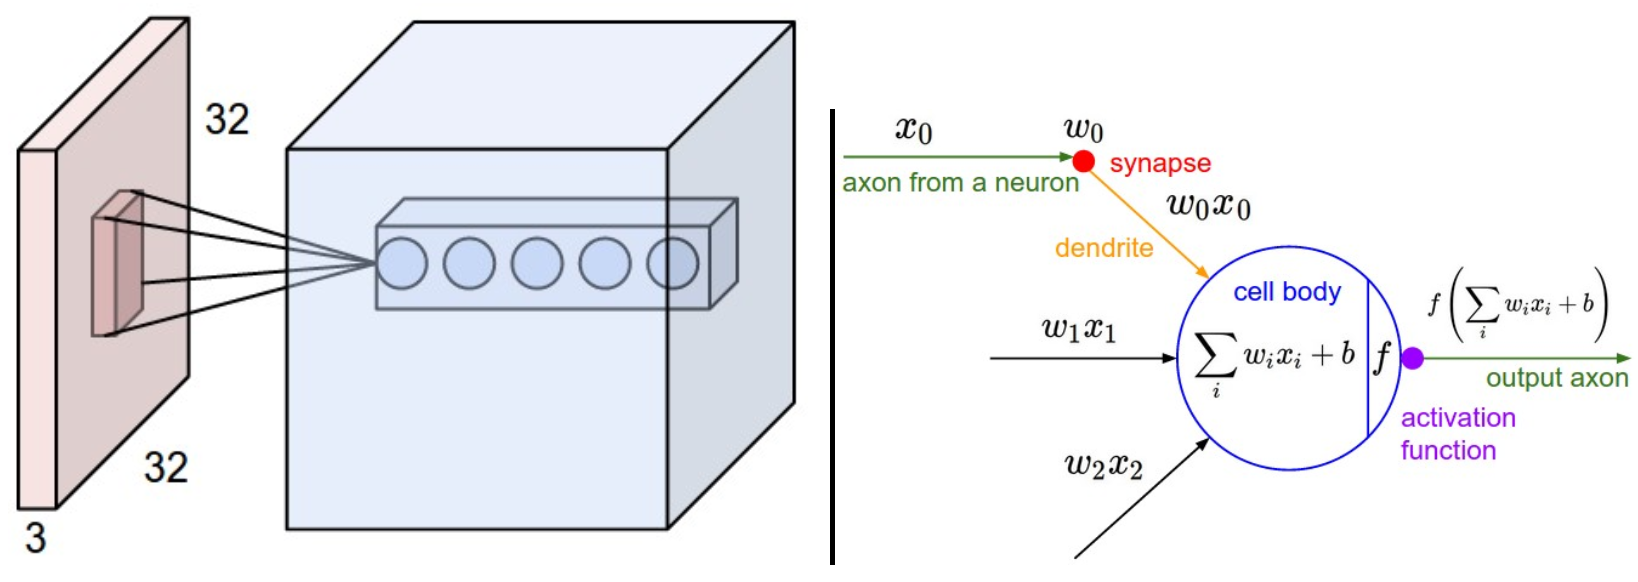
\includegraphics[scale=0.12]{/Users/pstey/projects_code/deep_learning_group/slides/intro_deep_learning/images/local_connectivity.png}
	\end{center}
	\end{frame}


	\begin{frame}{Convolutional Layer - Spatial Arrangement}
	
	\vspace{1em}
	\begin{columns}
	\column{\dimexpr\paperwidth-10pt}
	Number of Neurons in the Output Volume
	\begin{enumerate}
		\item \textbf{Depth (hyper-parameter):} Number of filters: Number of patterns to look for in input. Think back to steerable filters. The set of neurons looking at the same region may be referred to as \textbf{depth column} or \textbf{fiber}.
		\vspace{1em}
		\item \textbf{Stride (hyper-parameter):} Number of pixels used when sliding the filter. This controls the overlap between neurons. If stride is $1$, we move one pixel at a time (common, but depends on the width of filter).
		\vspace{1em}
		\item \textbf{Padding (hyper-parameter):} Number of zeros to add to the border of the volume. Convenient for convolution.
		
	\end{enumerate}
	\begin{center}
		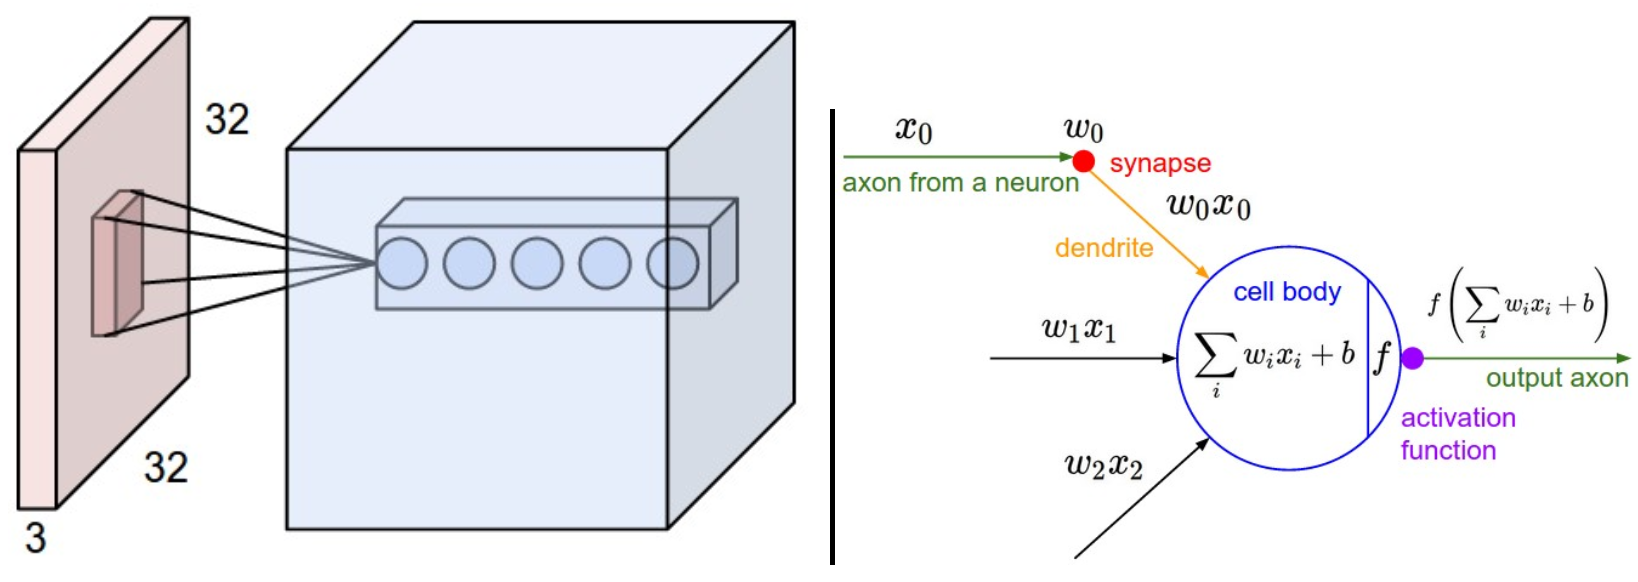
\includegraphics[scale=0.078]{/Users/pstey/projects_code/deep_learning_group/slides/intro_deep_learning/images/local_connectivity.png}
	\end{center}
	\end{columns}
	\end{frame}

	\begin{frame}
	\begin{center}
		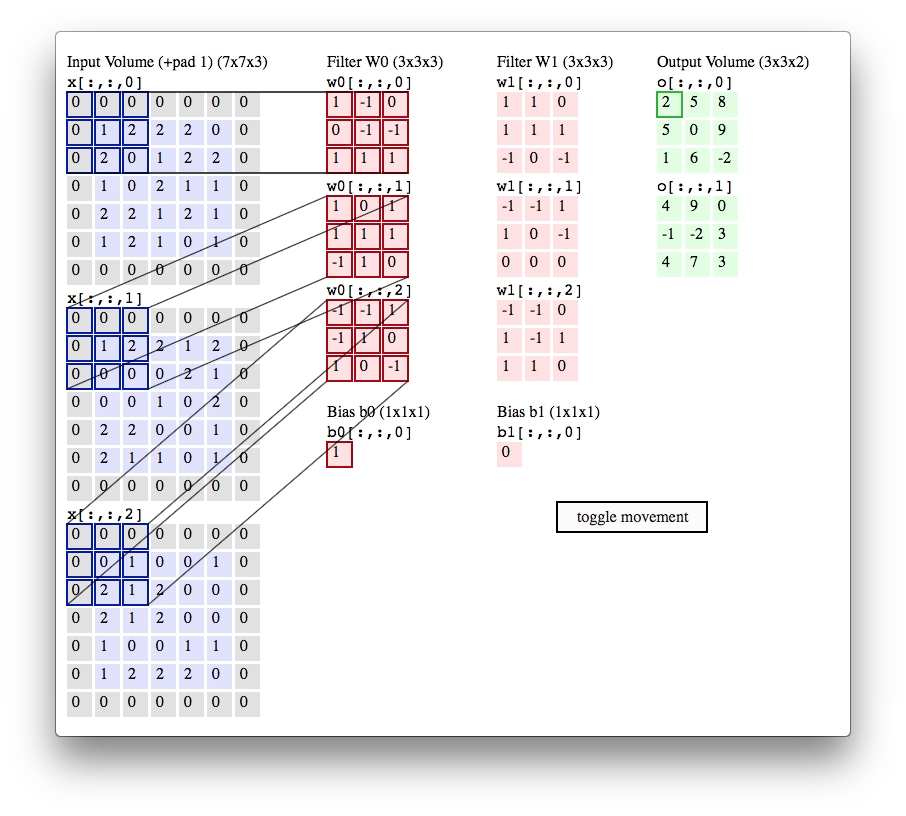
\includegraphics[scale=0.32]{/Users/pstey/projects_code/deep_learning_group/slides/intro_deep_learning/images/conv1.png}
	\end{center}
	\end{frame}
	
	\begin{frame}
	\begin{center}
		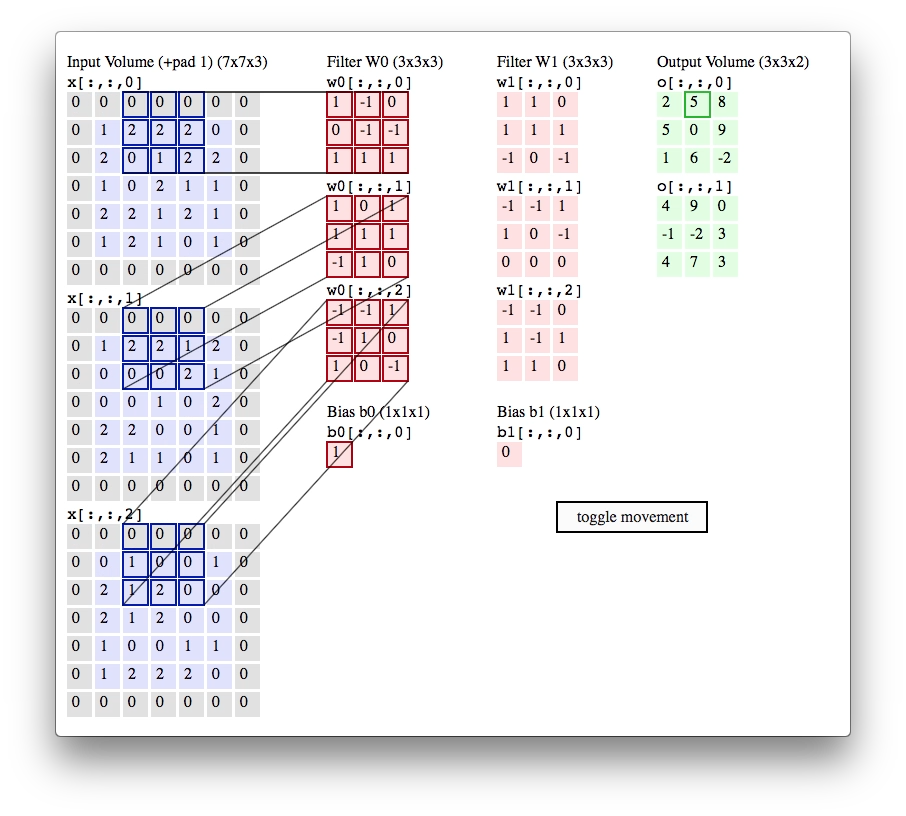
\includegraphics[scale=0.32]{/Users/pstey/projects_code/deep_learning_group/slides/intro_deep_learning/images/conv2.png}
	\end{center}
	\end{frame}
		
	\begin{frame}
	\begin{center}
		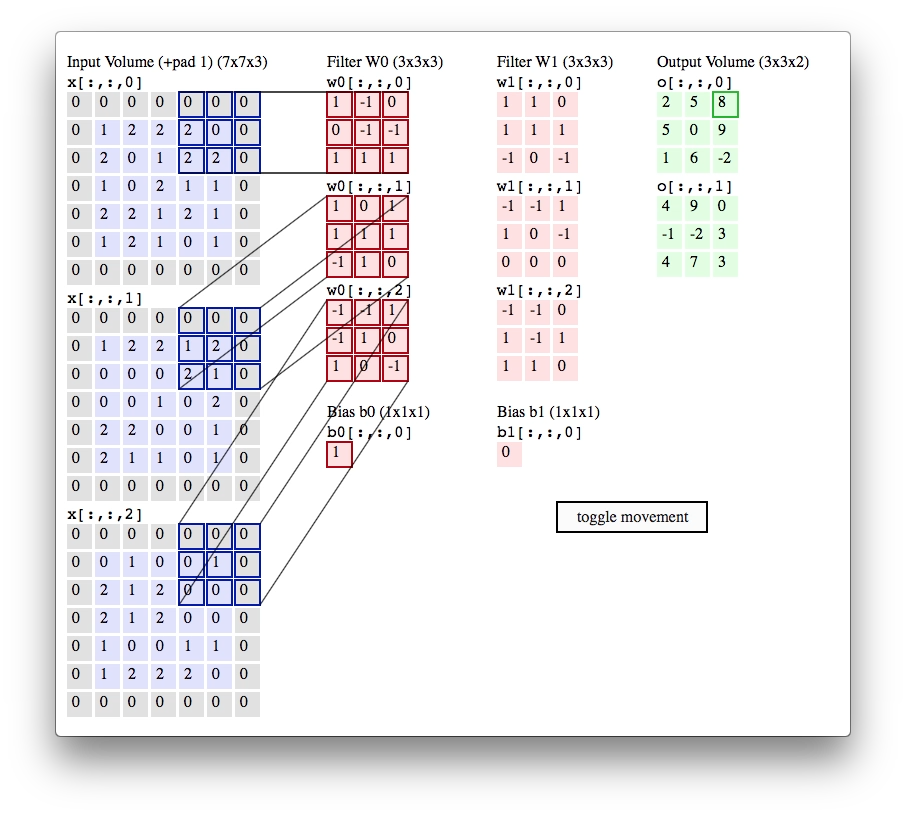
\includegraphics[scale=0.32]{/Users/pstey/projects_code/deep_learning_group/slides/intro_deep_learning/images/conv3.png}
	\end{center}
	\end{frame}
		
	\begin{frame}
	\begin{center}
		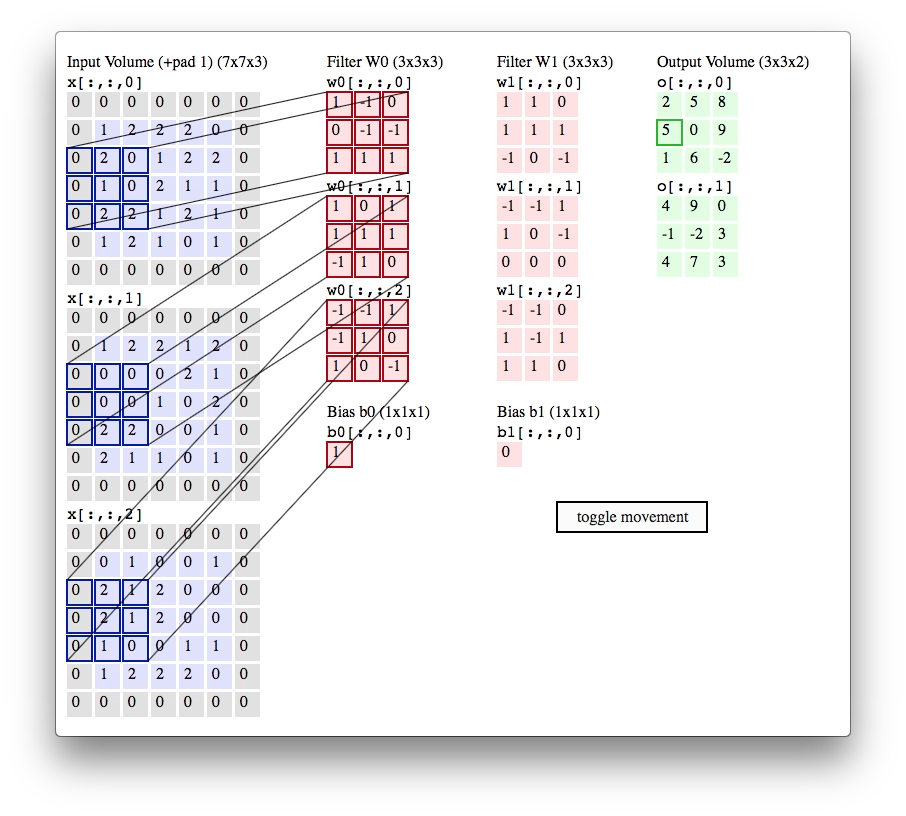
\includegraphics[scale=0.32]{/Users/pstey/projects_code/deep_learning_group/slides/intro_deep_learning/images/conv4.png}
	\end{center}
	\end{frame}

	\begin{frame}
	\begin{center}
		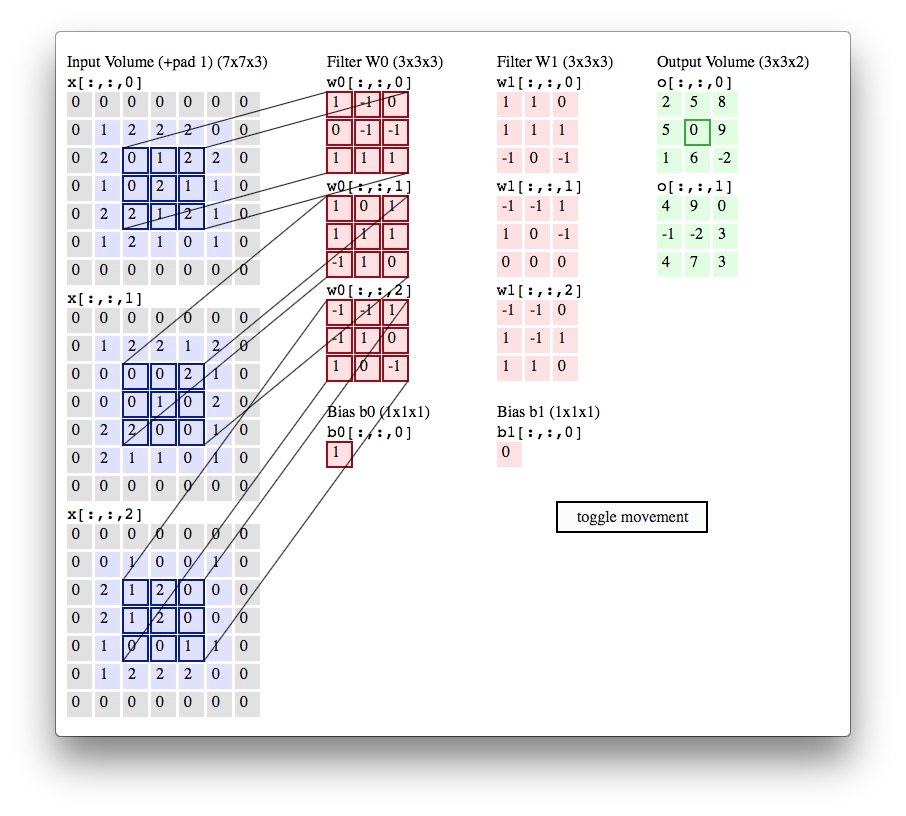
\includegraphics[scale=0.32]{/Users/pstey/projects_code/deep_learning_group/slides/intro_deep_learning/images/conv5.png}
	\end{center}
	\end{frame}
	
	\begin{frame}
	\begin{center}
		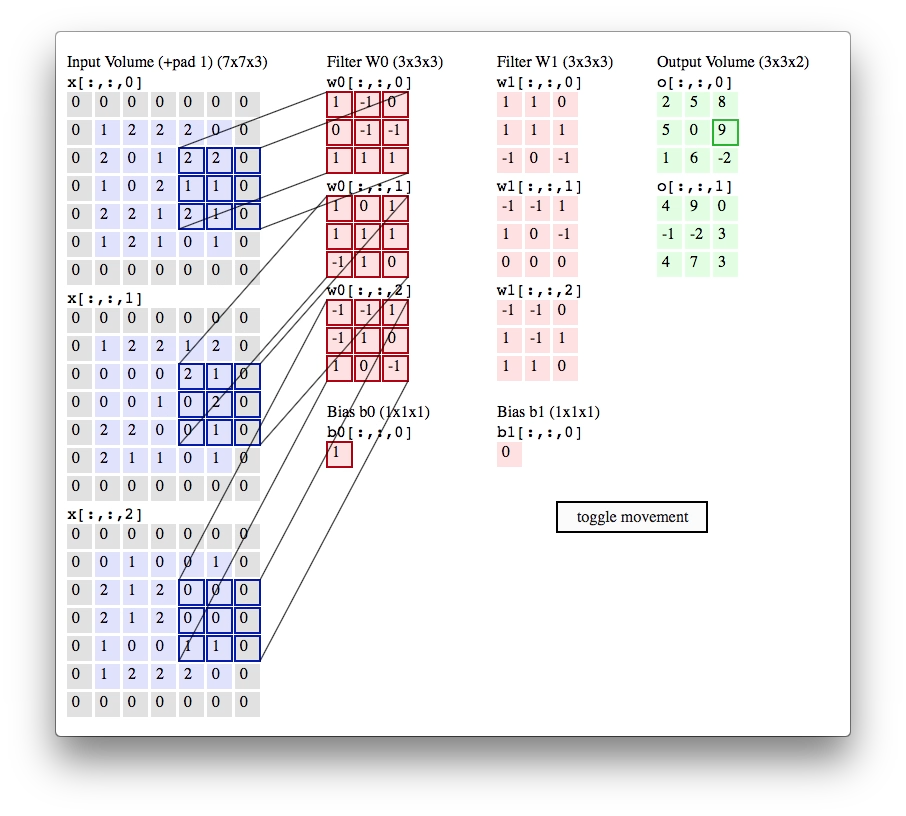
\includegraphics[scale=0.32]{/Users/pstey/projects_code/deep_learning_group/slides/intro_deep_learning/images/conv6.png}
	\end{center}
	\end{frame}
		
	\begin{frame}
	\begin{center}
		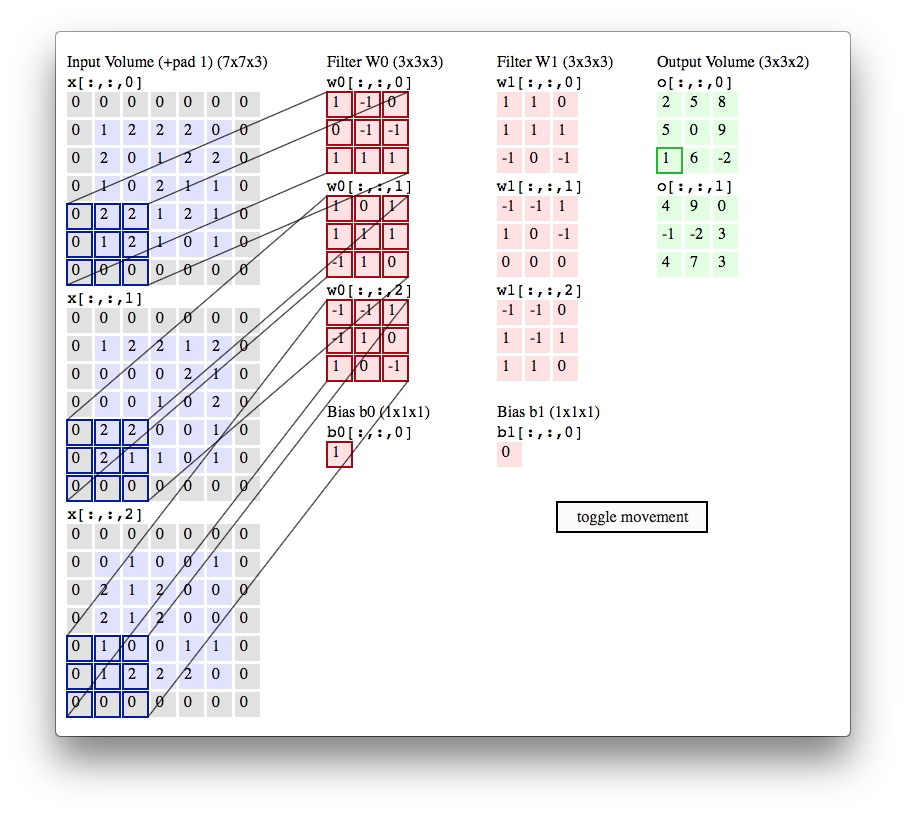
\includegraphics[scale=0.32]{/Users/pstey/projects_code/deep_learning_group/slides/intro_deep_learning/images/conv7.png}
	\end{center}
	\end{frame}
		
	\begin{frame}
	\begin{center}
		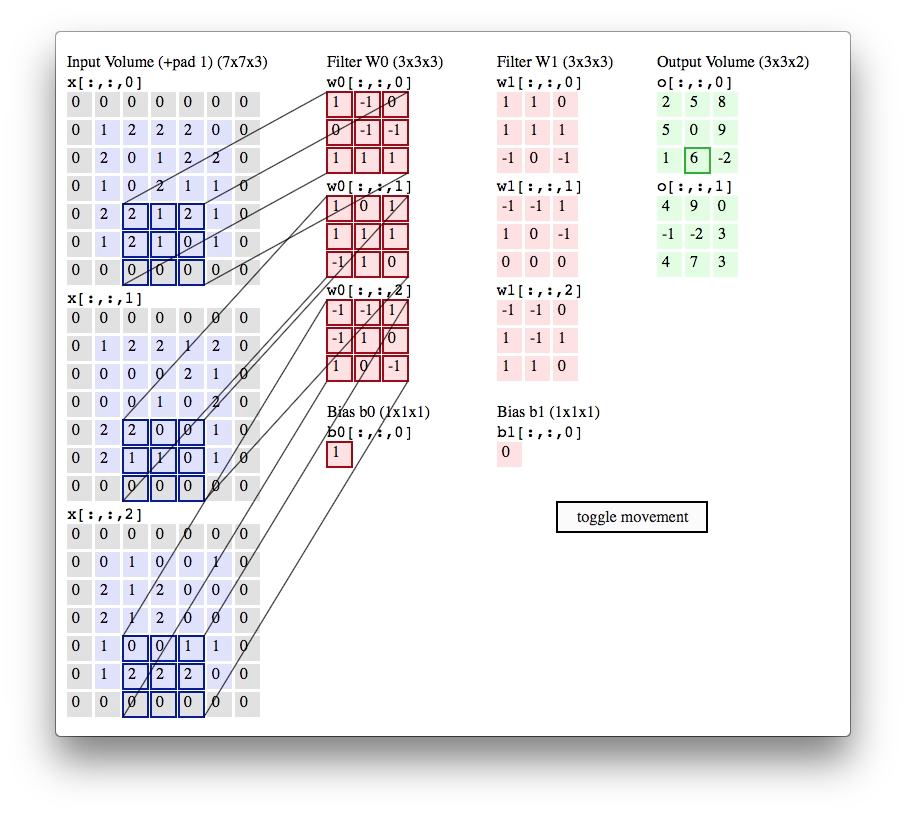
\includegraphics[scale=0.32]{/Users/pstey/projects_code/deep_learning_group/slides/intro_deep_learning/images/conv8.png}
	\end{center}
	\end{frame}


	\begin{frame}
	\begin{center}
		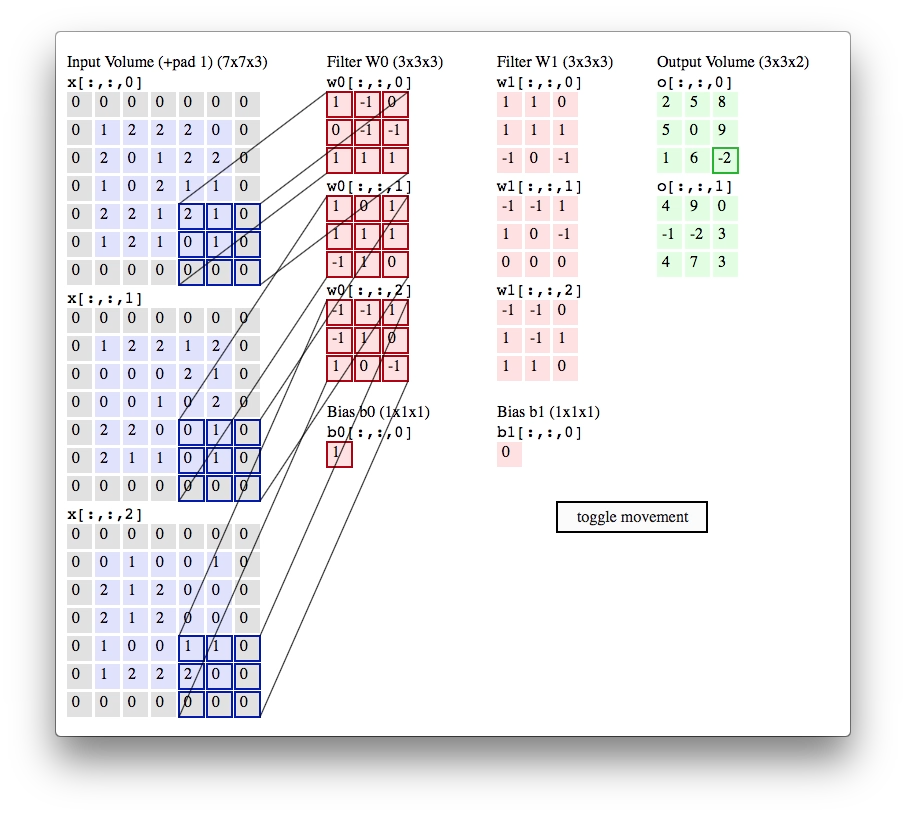
\includegraphics[scale=0.32]{/Users/pstey/projects_code/deep_learning_group/slides/intro_deep_learning/images/conv9.png}
	\end{center}
	\end{frame}
	
	\begin{frame}
	\begin{center}
		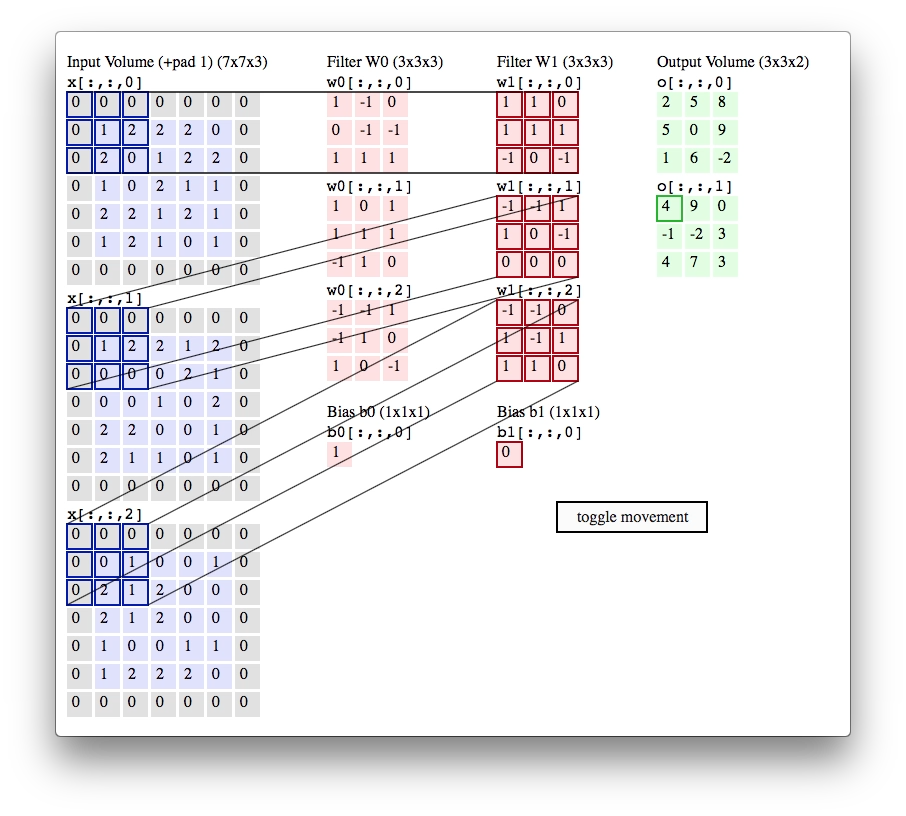
\includegraphics[scale=0.32]{/Users/pstey/projects_code/deep_learning_group/slides/intro_deep_learning/images/conv10.png}
	\end{center}
	\end{frame}
		
	\begin{frame}
	\begin{center}
		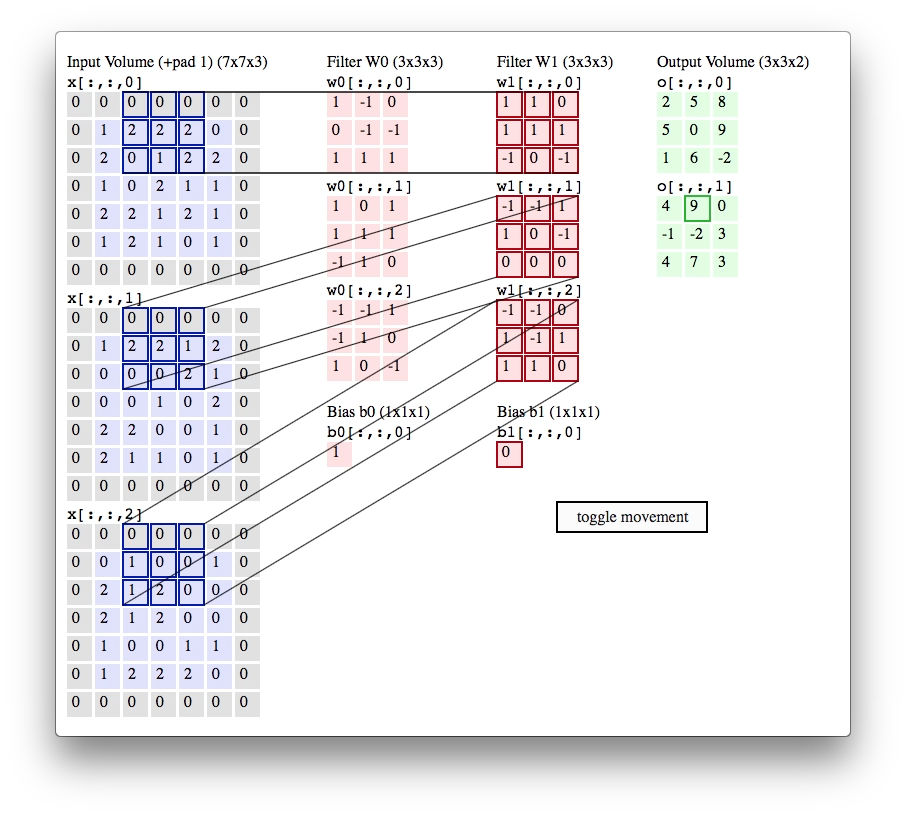
\includegraphics[scale=0.32]{/Users/pstey/projects_code/deep_learning_group/slides/intro_deep_learning/images/conv11.png}
	\end{center}
	\end{frame}
		
	\begin{frame}
	\begin{center}
		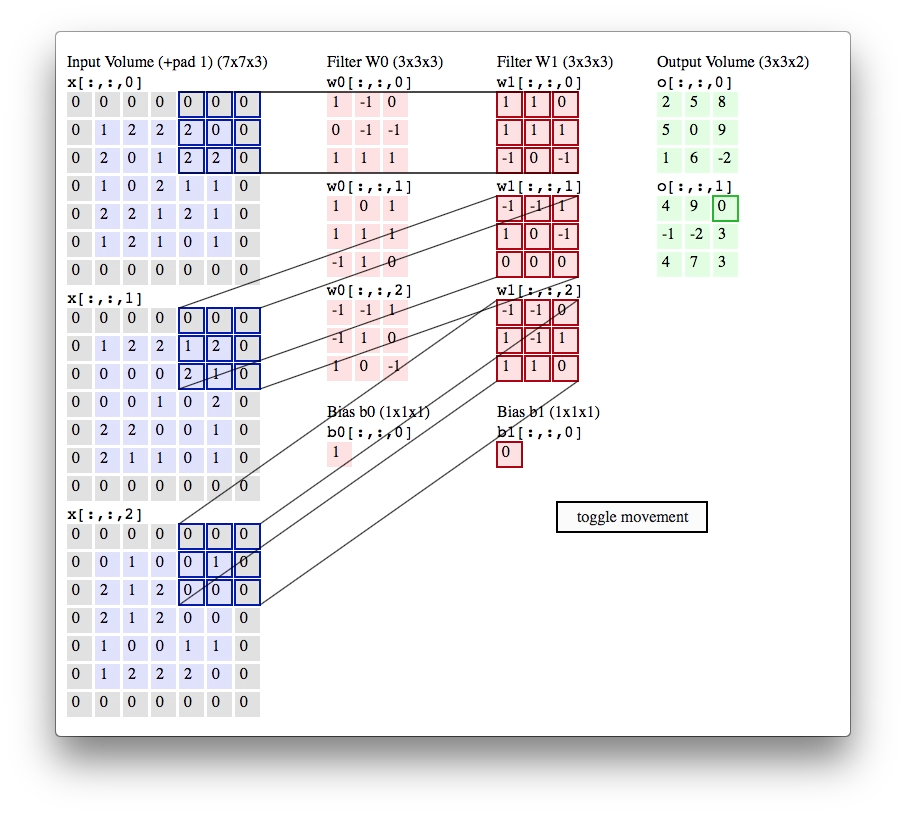
\includegraphics[scale=0.32]{/Users/pstey/projects_code/deep_learning_group/slides/intro_deep_learning/images/conv12.png}
	\end{center}
	\end{frame}

	\begin{frame}
	\begin{center}
		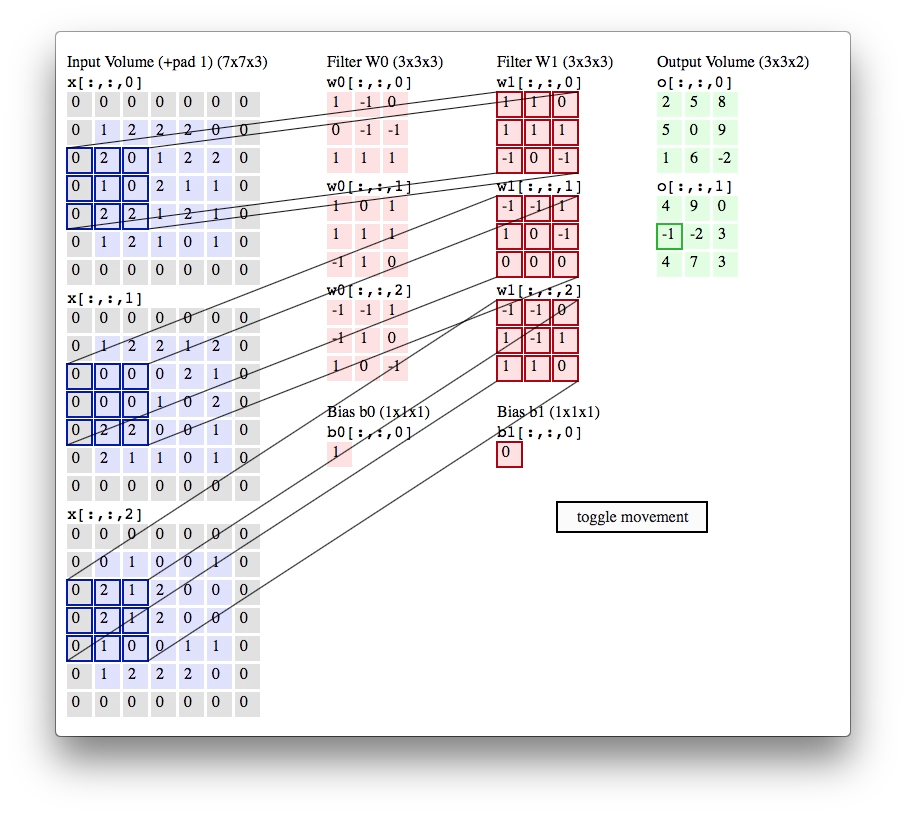
\includegraphics[scale=0.32]{/Users/pstey/projects_code/deep_learning_group/slides/intro_deep_learning/images/conv13.png}
	\end{center}
	\end{frame}
	
	\begin{frame}
	\begin{center}
		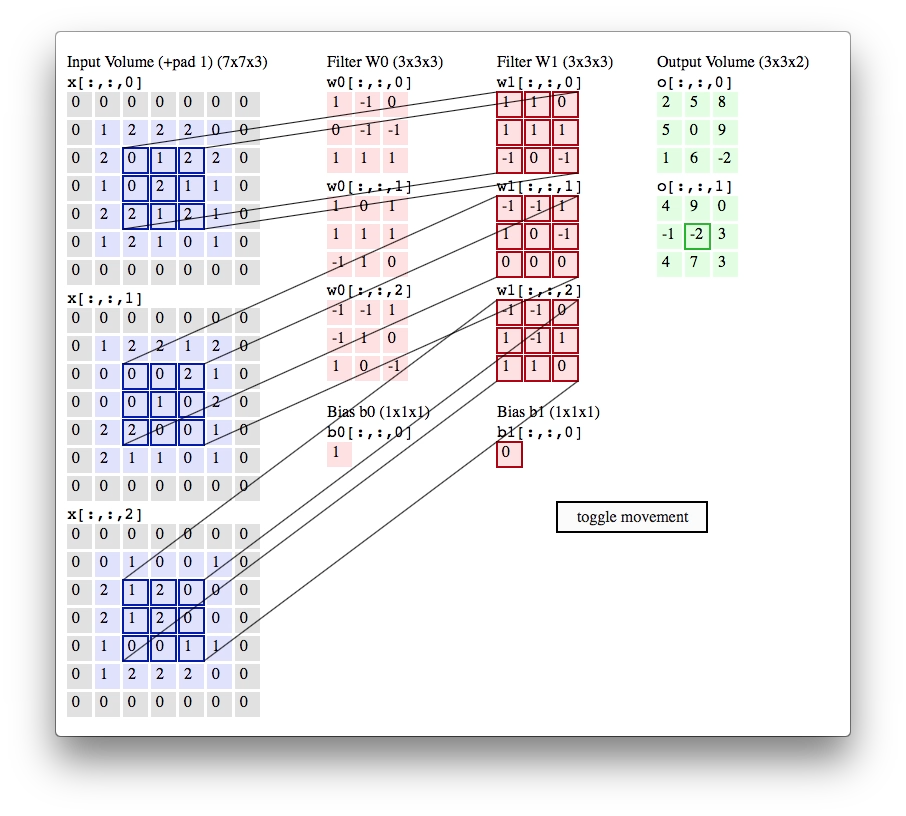
\includegraphics[scale=0.32]{/Users/pstey/projects_code/deep_learning_group/slides/intro_deep_learning/images/conv14.png}
	\end{center}
	\end{frame}
		
	\begin{frame}
	\begin{center}
		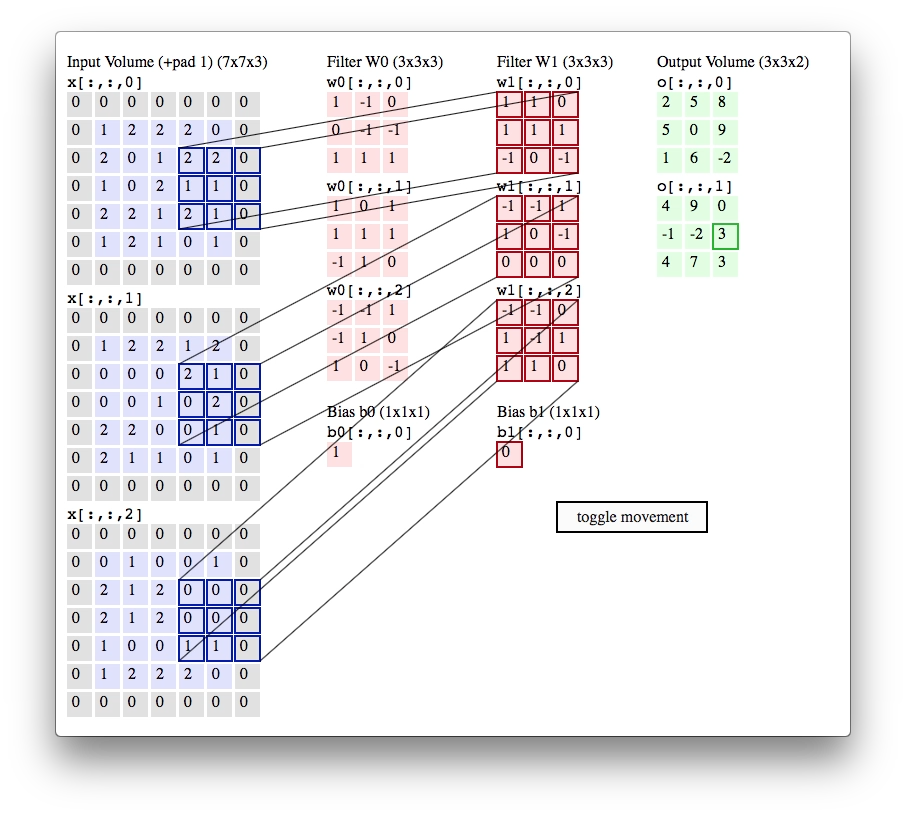
\includegraphics[scale=0.32]{/Users/pstey/projects_code/deep_learning_group/slides/intro_deep_learning/images/conv15.png}
	\end{center}
	\end{frame}
		
	\begin{frame}
	\begin{center}
		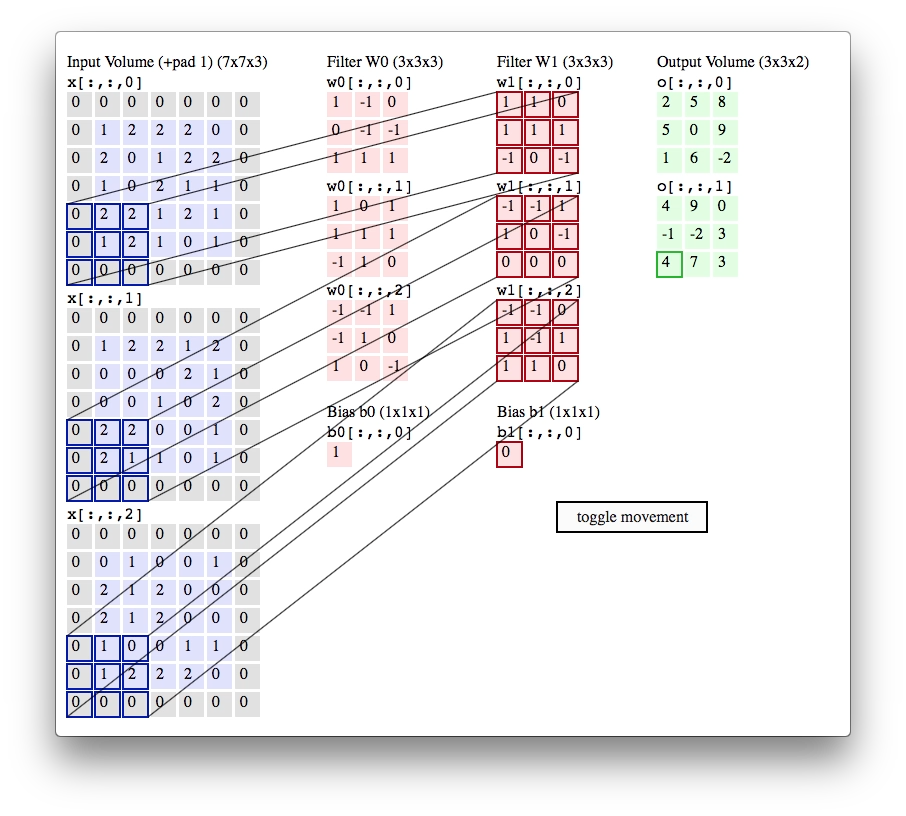
\includegraphics[scale=0.32]{/Users/pstey/projects_code/deep_learning_group/slides/intro_deep_learning/images/conv16.png}
	\end{center}
	\end{frame}

	\begin{frame}
	\begin{center}
		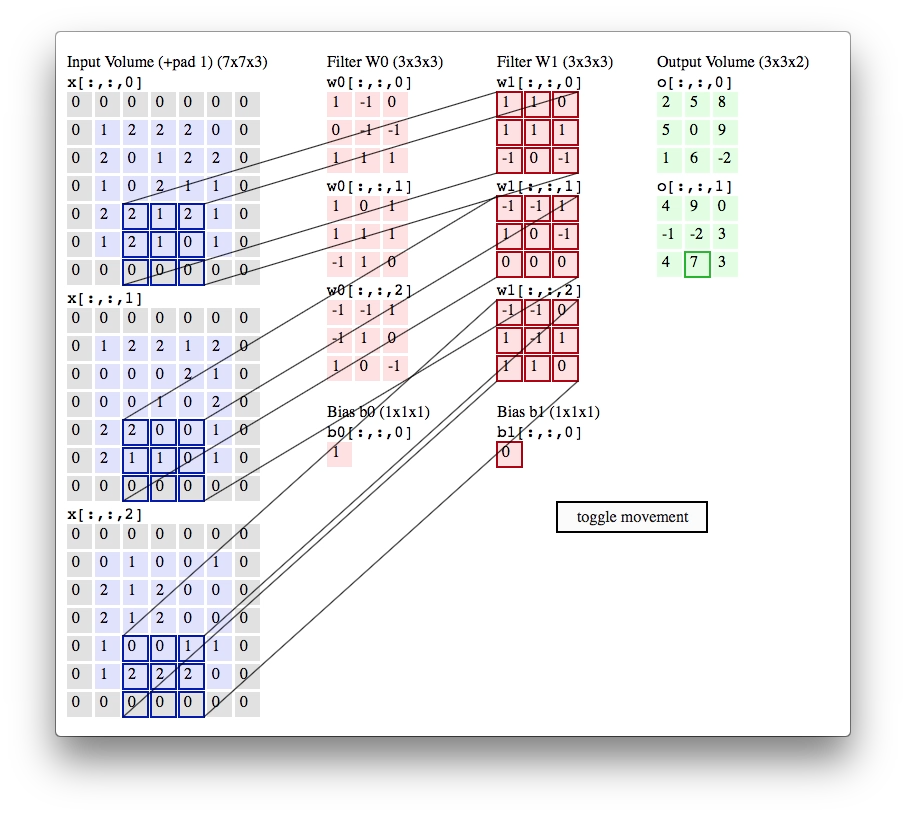
\includegraphics[scale=0.32]{/Users/pstey/projects_code/deep_learning_group/slides/intro_deep_learning/images/conv17.png}
	\end{center}
	\end{frame}
		
	\begin{frame}
	\begin{center}
		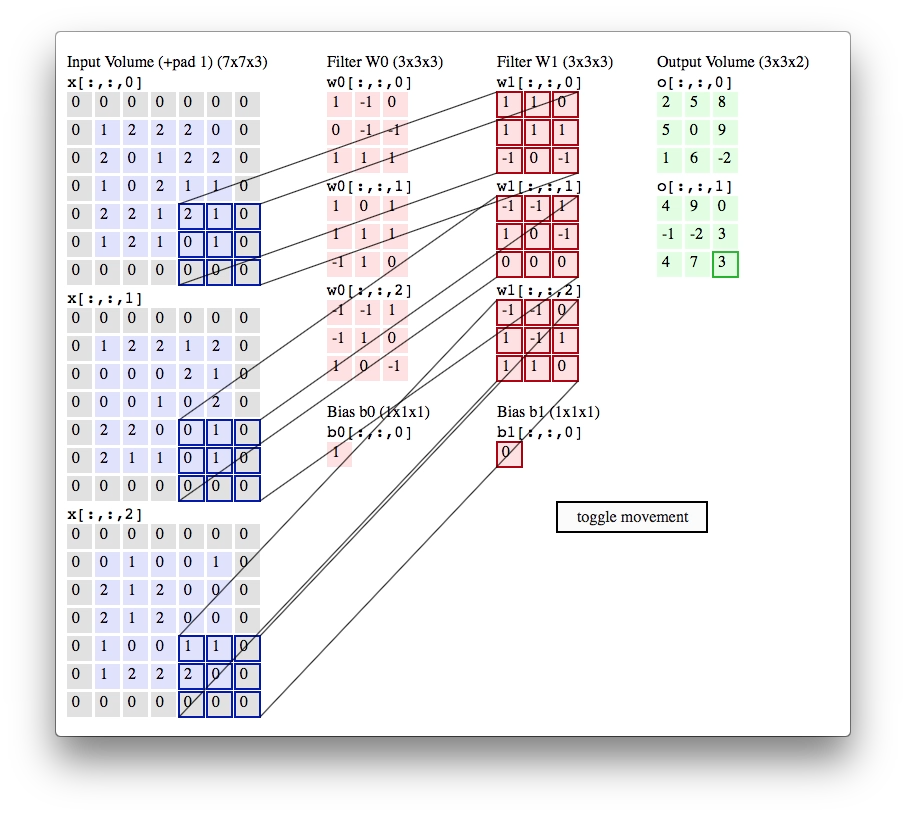
\includegraphics[scale=0.32]{/Users/pstey/projects_code/deep_learning_group/slides/intro_deep_learning/images/conv18.png}
	\end{center}
	\end{frame}

\subsection{Real-World Constraints}
	\begin{frame}{Mutual Constraints of Hyper-Parameters}
	\begin{enumerate}
		\item If stride is one, $S = 1$, it's common to set padding, $P = \frac{F-1}{2}$, to ensure that input and output volumes have the same size. 
		\vspace{1em}
		\item The number of neurons that fit is $\frac{W - F + 2P}{S} + 1$. Must set hyper-parameters so there number of neurons is an integer!
		\vspace{1em}
		\item \textbf{Real-World Example:} (Winner of ImageNet 2012) Images $227 \times 227 \times 3$, $F = 11$, $S = 4$, $P = 0$, $K = 96$.
			\begin{itemize}
				\vspace{1em}
				\item Number of neurons in \textit{first layer}
				\begin{enumerate}[]
				
					\item $\frac{227 - 11}{4} + 1 = 55$ (per width) 
									\vspace{0.5em}
					\item $55 \times 55 \times 96 = 290400$ (width $\times$ height $\times$ depth)
									\vspace{0.5em}
					\item Each neuron has $11 \times 11 \times 3 = 363$ weights plus $1$ bias
									\vspace{0.5em}
					\item $290400 \times 364 = 105705600$ parameters \textit{in the first layer!}
				\end{enumerate}
			\end{itemize}
	
	\end{enumerate}
	\end{frame}
	
	\begin{frame}{Parameter Sharing}
	\textbf{If one feature (filter/kernel/depth slice) is useful at pixel $(x_1, y_1)$, then it is also useful at pixel $(x_2, y_2)$}
	
	\begin{enumerate}
		\item All neurons in the same depth slice have same weights and bias.
		\item Example before $96 \times 11 \times 11 \times 3 = 34848$ unique weights $ + 96 $ biases $ = 34944$ parameters
		\item Then forward pass can be seen as the convolution of that slice neuron's weights with the input volume.
		\item Weights $=$ filter/kernel that is convolved with the input
	\end{enumerate}
	
	\begin{columns}
	\begin{column}{0.7\textwidth}
	\begin{center}
		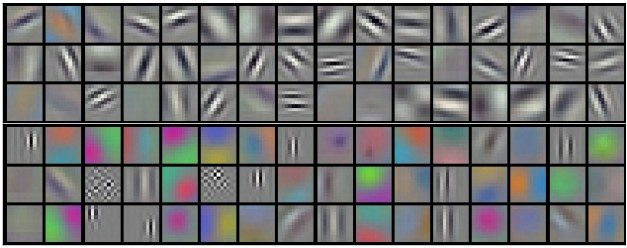
\includegraphics[scale=0.25]{/Users/pstey/projects_code/deep_learning_group/slides/intro_deep_learning/images/weights.jpeg}
	\end{center}
	\end{column}
	\begin{column}{0.3\textwidth}
		\tiny{Example filters learned by Krizhevsky et al. Each of the 96 filters shown here is of size $11 \times 11 \times 3$}
	\end{column}
	
	\end{columns}
	\end{frame}

\subsection{Pooling Layer}
	\begin{frame}{Pooling Layer}
	\begin{enumerate}
		\item Inserted in-between convolutional layers
		\item Goal: To reduce spatial size, amount of parameters, computation requirements, and overfitting
		\item Operates independently on every depth slice and resizes spatially using $max(\cdot)$ (or could be $mean(\cdot)$ or $L2$)
		\item Introduces no parameters, since it is a fixed operation
		\item Hyper-parameters: $F$ (spatial size) and $S$ (stride)
	\end{enumerate}
	\begin{columns}
	\begin{column}{0.25\textwidth}
	\begin{center}
		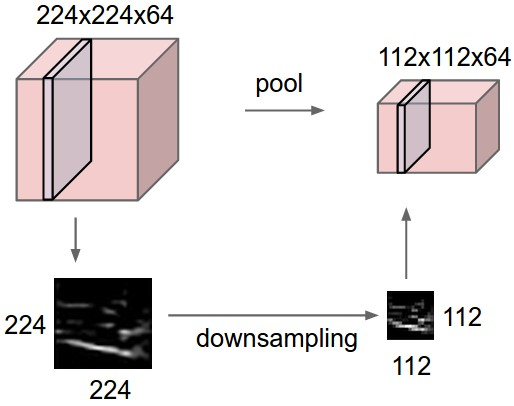
\includegraphics[scale=0.23]{/Users/pstey/projects_code/deep_learning_group/slides/intro_deep_learning/images/pool.jpeg}
	\end{center}
	\end{column}
	\begin{column}{0.75\textwidth}
	\begin{center}
		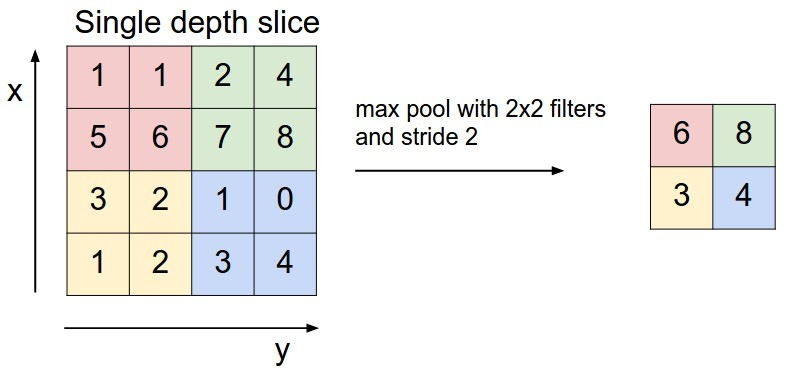
\includegraphics[scale=0.22]{/Users/pstey/projects_code/deep_learning_group/slides/intro_deep_learning/images/maxpool.jpeg}
	\end{center}
	\end{column}
	
	\end{columns}

	\end{frame}
	
\subsection{Normalization Layer}
	\begin{frame}{Normalization Layer}
	
	\textbf{Future - Hope of Getting Rid of Pooling}
	\vspace{1em}
		\begin{enumerate}
			\item Striving for Simplicity: Newer works propose discarding pooling. Suggest using larger strides
			\item Variational auto-encoders
			\item Generatie Adversarial Networks
		\end{enumerate}
	\vspace{2em}
	\textbf{Normalization Layer}
		\begin{enumerate}
			\item Have show no real advantages
		\end{enumerate}
	\end{frame}
	
	
	\begin{frame}{Practice}
	\textbf{Hyper-Parameters and Layer Sizing}
	\vspace{1em}
	\begin{enumerate}
		\item Input layer should be divisible by 2 many times
		\vspace{0.5em}
		\item Conv layer use small filters $(3 \times 3)$, $(5 \times 5)$, (notice odd) and stride $S = 1$ (reduce sizing headaches - downsampling done by pooling)
		\vspace{0.5em}
		\item Use padding that doesn't alter dimension
		\vspace{0.5em}
		\item Pool layers $(2 \times 2)$, $F = 2$, and $S = 2$. Discards $75\%$ of activations
		\vspace{0.5em}
		\item Compromise based on memory constraints (GPU). May have to sacrifice at the 1st layer.
	\end{enumerate}
	\end{frame}

	\begin{frame}{Popular Networks}
	\begin{enumerate}
		\item LeNet: LeCun 90's - read zip code (first successful ConvNet)
		\vspace{0.5em}
		\item AlexNet: Alex Krizhevsky, Ilya Sutskever, and Geoff Hinton. Popularize ConvNets for computer vision. ImageNet. Deeper, bigger than LeNet
		\vspace{0.5em}
		\item ZF Net: Matthew Zeiler and Rob Fergus. ILSVRC 2013 Winner. Improved by expanding the size of the middle convolutional layers making the stride and filter size on the first layer smaller
		\vspace{0.5em}
		\item GoogLeNet: Szegedy et al. from Google. ILSVRC 2014 winner. Reduced the number of parameters in the network from 60M to 4M (inception model)
		\vspace{0.5em}
		\item ResNet: Residual Network. Kaiming He et al. ILSVRC 2015 winner. It features special skip connections and heavy use of batch normalization. State of the art as of 2016 
	\end{enumerate}
	\end{frame}
	
	
	
	
	
\section{RNNs}

\subsection{RNNs and LSTMs}

	\begin{frame}{Recurrent Neural Networks (RNNs)}

		RNNs are a type of neural network that share parameters across time. They are used frequently for natural language processing (NLP) and time series data.

	\end{frame}

	\begin{frame}{RNNs}
	\begin{enumerate}
		\item Unlike standard neural networks or CNNs, RNNs introduce a temporal or sequential component to the system.
		\item While CNNs introduce idea of spatial dependence, RNNs rely on the notion that \textit{the current input relies on previous inputs} 
	\end{enumerate}
	\begin{center}
		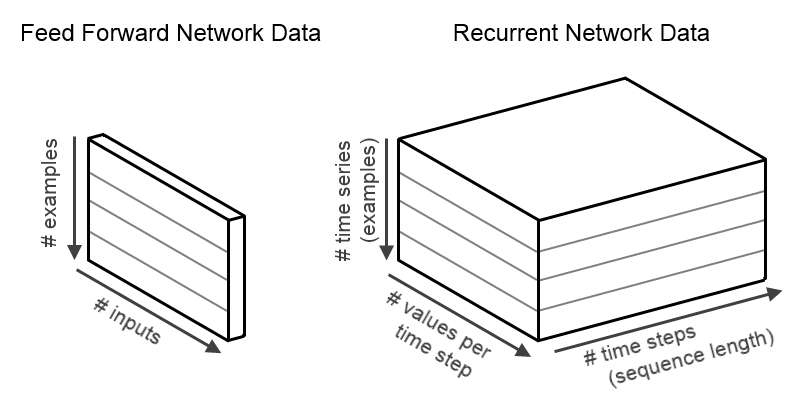
\includegraphics[scale=0.35]{/Users/pstey/projects_code/deep_learning_group/slides/intro_deep_learning/images/rnn_data.png}
	\end{center}
	\end{frame}


	\begin{frame}{RNN Architecture and Notation}
	\begin{enumerate}
		\item Current input: $x_t$
		\item Current hidden state: $h_t$
		\item Non-linear activation function $\sigma$ or $tanh$
		\item Predicted output: $\widehat{y_t}$
	\end{enumerate}
	
	\begin{center}
		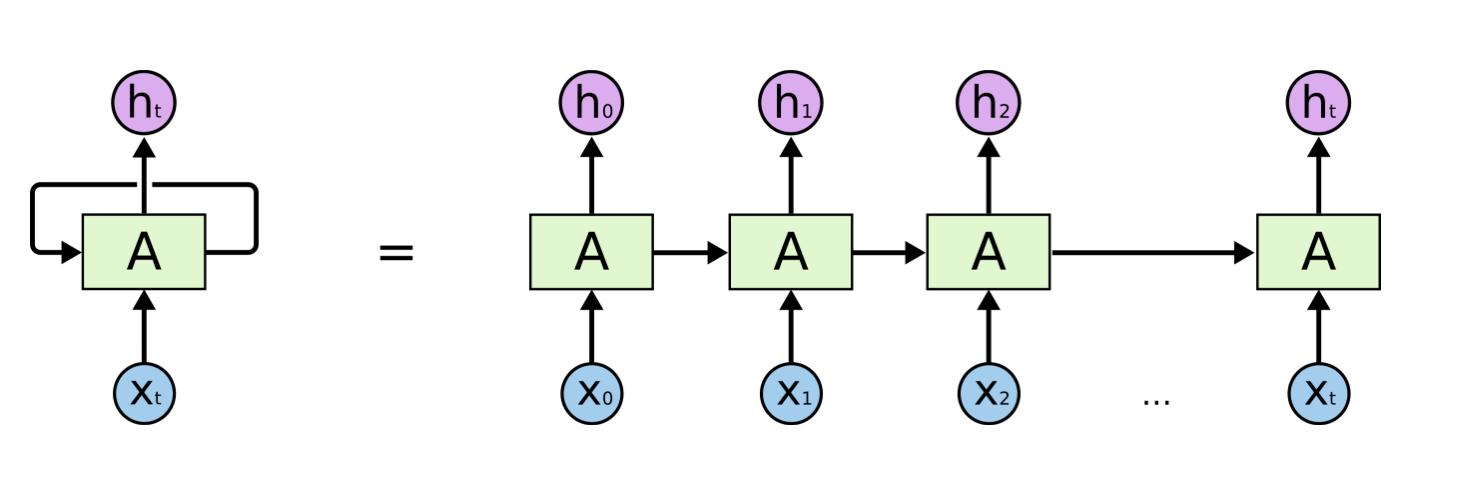
\includegraphics[scale=0.2]{/Users/pstey/projects_code/deep_learning_group/slides/intro_deep_learning/images/rnn_unrolled2.png}
	\end{center}
	\end{frame}
	
	
	
	
	\begin{frame}{Long-Term Dependencies}
	\begin{enumerate}
		
		\item Suppose we want a model that predicts the next word in this sentence: 
		\begin{itemize}
			\item ``\textit{The clouds are in the} \texttt{<WORD>}''
		\end{itemize}
		\vspace{2em}
		
		\item Now suppose we to model the next word in this sentence: 
		\begin{itemize}
			\item ``\textit{I grew up in France and lived there most of my life. As a result I am a native speaker of} \texttt{<WORD>}''
		\end{itemize}
	\end{enumerate}
	
	\begin{center}
		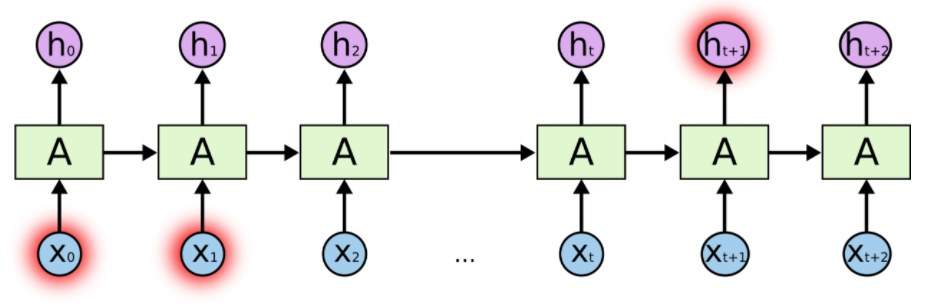
\includegraphics[scale=0.2]{/Users/pstey/projects_code/deep_learning_group/slides/intro_deep_learning/images/long_depend.png}
	\end{center}
	\end{frame}

	\begin{frame}{Long Short Term Memory Networks (LSTM)}
		LSTMs are a species of RNN that is designed for learning long-term dependencies. While standard RNNs are able to model temporal dependencies, LSTMs have a much more elaborate structure.
		
	\begin{columns}
	\begin{column}{0.5\textwidth}
	\begin{center}
		\vspace{-4em}
		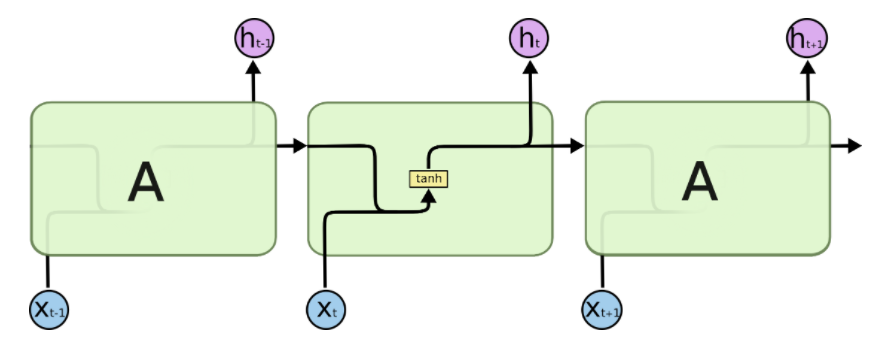
\includegraphics[scale=0.19]{/Users/pstey/projects_code/deep_learning_group/slides/intro_deep_learning/images/standard_rnn.png}
	\end{center}
	\end{column}
	
	\begin{column}{0.5\textwidth}
	\begin{center}
		\vspace{7em}
		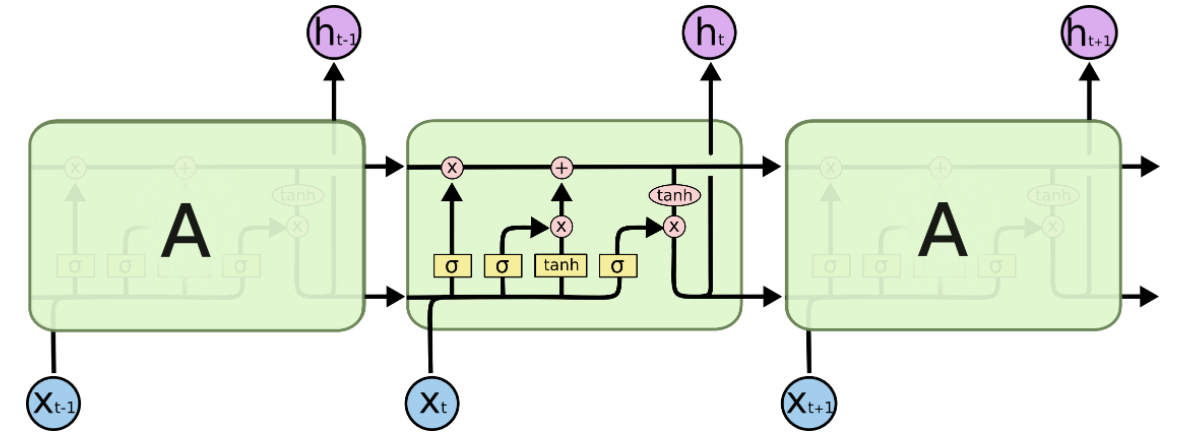
\includegraphics[scale=0.14]{/Users/pstey/projects_code/deep_learning_group/slides/intro_deep_learning/images/lstm.png}
	\end{center}
	\end{column}
	\end{columns}
	\end{frame}

	\begin{frame}{Cell State}
	The key idea of LSTMs is that of cell state to propagate information.
	\vspace{2em}
	\begin{enumerate}
		\item Cell state is subject to linear operations
		\item Information in cell state can be ``forgotten'' using a system of gates
	\end{enumerate}
	\begin{center}
		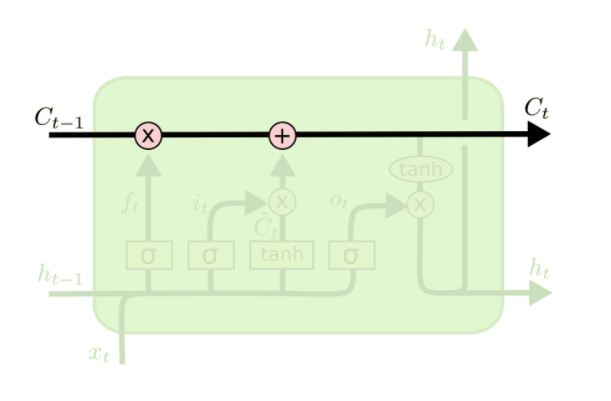
\includegraphics[scale=0.3]{/Users/pstey/projects_code/deep_learning_group/slides/intro_deep_learning/images/lstm_cell_state.png}
	\end{center}
	\end{frame}
	
	
	\begin{frame}{LSTM Forget Gate Layer}
	Forget gate layer is a sigmoid layer that decides the values to be updated with
	\[
	f_t = \sigma(W_f \cdot [h_{t-1}, x_t] + b_f)
	\]
	\begin{enumerate}
		
		\item This layer looks at $h_{t-1}$ and $x_t$ and updates the cell state
		\item $f_t$ has range $(0, 1)$
		\item $0$ indicates ``complete get rid of this'', and $1$ indicates ``completely keep this''.
	\end{enumerate}
	\begin{center}
		\includegraphics[scale=0.14]{/Users/pstey/projects_code/deep_learning_group/slides/intro_deep_learning/images/lstm_forget_gate.png}
	\end{center}
	\end{frame}
	
	
	
	\begin{frame}{Input Gate Layer}
	Input gate layer is a combination of a sigmoid layer and $tanh$ layer that decide the new information to keep with
	\[
	i_t = \sigma(W_i \cdot [h_{t-1}, x_t] + b_i) 
	\]
	\[
	\widetilde{C}_t = \text{tanh}(W_C \cdot [h_{t-1}, x_t] + b_C)
	\]
	\begin{enumerate}
		
		\item Sigmoid layer is our ``input gate layer''
		\item $tanh$ layer creates candidate values
				
	\end{enumerate}
	\begin{center}
		\includegraphics[scale=0.15]{/Users/pstey/projects_code/deep_learning_group/slides/intro_deep_learning/images/lstm_tanh_layer.png}
	\end{center}
	\end{frame}
	

	
	\begin{frame}{Update the Cell State}
	Now we update the cell state using
	\[
	C_t = f_t \cdot C_{t-1} + i_t \cdot \widetilde{C}_t
	\]
	\begin{enumerate}

		\item Multiply old state by $f_t$, forgetting what we had decided 
		\item And add $i_t \cdot \widetilde{C}_t$, our new candidate values
	\end{enumerate}
	\begin{center}
		\includegraphics[scale=0.15]{/Users/pstey/projects_code/deep_learning_group/slides/intro_deep_learning/images/lstm_3rd_layer.png}
	\end{center}
	\end{frame}
	



	\begin{frame}{Output Layer}
	Now we decide what to output with
	\[
	o_t = \sigma(W_o \cdot [h_{t-1}, x_t] + b_o) 
	\]
	\[
	h_t = o_t \cdot \text{tanh}(C_t)
	\]
	\begin{enumerate}

		\item Take updated cell state to help compute output 
		\item Apply sigmoid layer and $tanh$ layer
	\end{enumerate}
	\begin{center}
		\includegraphics[scale=0.15]{/Users/pstey/projects_code/deep_learning_group/slides/intro_deep_learning/images/lstm_4th_layer.png}
	\end{center}
	\end{frame}
	




\section{Autoencoders}

\subsection{Autoencoder Basics}
		\begin{frame}{Autoencoder Basics}
		\begin{enumerate}
			
			\item Feed-forward neural network
			\item Used for unsupervised learning 
			\item Trained to reproduce input layer in the output layer
			\item Training uses gradient descent
		\end{enumerate}
		\end{frame}
		

		\begin{frame}{Autoencoder Basics cont.}
		\begin{enumerate}
			\item Similar to PCA*, but more flexible  
			\item Autoencoders can accommodate non-linear transformations
			\begin{enumerate}[1]
				\item Consequence of flexible activation functions
				\item Turns out to be hugely useful 
			\end{enumerate}
		\end{enumerate}
		
		\vspace{8em}
		{\tiny * Actually, with squared error loss and no sigmoid transformation, it is equivalent to PCA (Baldi \& Hornik, 1989)}
		\end{frame}
		
		\begin{frame}{Simple Autoencoder}
		\begin{figure}
			\includegraphics[scale = 0.20]{/Users/pstey/projects_code/deep_learning_group/slides/intro_deep_learning/images/autoencoder.png}
		\end{figure}	
		\end{frame}
	
		\begin{frame}{Simple Autoencoder cont.}
		
		From input layer to hidden layer is``encoder'':
		\vspace{-1em}
		\begin{center}
		$$ f(x) = \sigma(Wx + b) $$
		\end{center}
		Hidden layer to the output is the ``decoder'':
		\vspace{-1em}
		\begin{center}
		$$ g(x) = \sigma(W'x + b') $$
		\end{center}
		where $\sigma$ is the activation function (often sigmoid) and $W'$ is often $W^\top$ (known as having ``tied'' weights).
		\end{frame}
		
		\begin{frame}{Simple Autoencoder cont.}
		\begin{enumerate}
			\item Input layer $\rightarrow$ hidden layer (fewer units) $\rightarrow$ output layer  
			\item Hidden layers values can be thought of as lossy compression of input layer
			\item Hidden layer with fewer units than input is often called ``bottleneck'' or under-complete layer

		\end{enumerate}
		\end{frame}
		
		
		\begin{frame}{Question}
		In a sense, autoencoders want to learn an approximation to the identity function.
			\begin{center}
				Why would this be useful?
			\end{center}
		\end{frame}
		
		\begin{frame}{Answer}
		This turns out to have several practical uses.
		\vspace{2em}
		\begin{enumerate}
			\item Autoencoders learn a kind of latent representation of the input
			\item Can be used for initializing weights and biases prior to fitting neural net
			\item Very well suited to dimensionality reduction in NLP tasks 
		\end{enumerate}
		\end{frame}

	
		

		
\subsection{Stacked and Denoising Autoencoders}
		\begin{frame}{Stacked Autoencoder}
		\begin{enumerate}
			\item Sometimes called deep autoencoder
			\item Feed-forward neural network
			\item Has additional layers 
			\item Still ``unsupervised'' in the sense of no labels or real-valued outcome variable
			\item Output layer is still $\hat{x}$
			\item Trained in stages
		\end{enumerate}
		\end{frame}
		
		\begin{frame}{Stacked Autoencoder}
		\begin{figure}
			\includegraphics[scale = 0.20]{/Users/pstey/projects_code/deep_learning_group/slides/intro_deep_learning/images/stacked_autoencoder.png}
		\end{figure}	
		\end{frame}
		
		\begin{frame} {Stacked Autoencoder cont.}
		\begin{enumerate}
			\item Beneficial for data with hierarchical organization
			\item Can be difficult to train using back propagation 
		\end{enumerate}
		\end{frame}



			\begin{frame}{Denoising Autoencoder}
			\begin{enumerate}
				\item Stochastic version of autoencoder
				\item Random noise injected into the input layer
				\begin{enumerate}[1]
					\item \textit{Masking noise}: some fraction of elements* in $x$ set to $0$ 
					\item \textit{Gaussian additive noise}: $\tilde{x}|x \sim \mathcal{N}(x, \sigma^2I) $
					\item \textit{Salt-and-pepper noise}: fraction of elements* in $x$ set to either min or max possible value (often $0$ or $1$) according to coin toss
				\end{enumerate}
			\end{enumerate}
			\vspace{5em}
			\hspace{2em} {\tiny * chosen at random for each example}
			\end{frame}
			
	
			
			\begin{frame}{Denoising Autoencoder}
			\begin{enumerate}
				\item Output layer is evaluated against original (uncorrupted) data
				\item Goal is slightly different from simple autoencoder
				\begin{enumerate}[1]
					\item Not attempting to learn identity function
					\item We want robustness of representation
					\item Learned representation is insensitive to perturbations in the input
				\end{enumerate}
			\end{enumerate}
			\end{frame}
			
						
			
			\begin{frame}{Denoising Autoencoder}
			\begin{figure}
				\includegraphics[scale = 0.25]{/Users/pstey/projects_code/deep_learning_group/slides/intro_deep_learning/images/denoising_autoencoder2.png}
			\end{figure}	
			\end{frame}
	

			\begin{frame}{Denoising Autoencoder cont.}
			\begin{enumerate}
				\item Training proceeds fairly similarly to standard autoencoder 
				\item Crucial difference is the loss function is calculated using \textit{uncorrupted} input layer 
			\end{enumerate}
			\end{frame}
			

		\begin{frame} {Extending Denoising Autoencoder}
		\begin{enumerate}
			\item Some noise types only corrupt subset of the input's components 
			\begin{enumerate}[1]
				\item Masking noise
				\item Salt-and-pepper noise
			\end{enumerate}
			\item For these, we can extend denoising by adding emphasis on corrupted components.
			\item Use hyperparameters $\alpha$ and $\beta$ to control emphasis; for squared error loss, this yields
		
			$$ L(x, \hat{x}) = \alpha \left( \sum_{i \in \mathcal{I}(\tilde{x})} \left(x_i - \hat{x}_i \right) \right)   + \beta \left( \sum_{i \notin \mathcal{I}(\tilde{x})} \left(x_i - \hat{x}_i \right) \right)$$
			where $ \mathcal{I}(\tilde{x}) $ denotes indexes components of $x$ that were corrupted.
		\end{enumerate}
		\end{frame}




\section{Summary}

\subsection{When to use Neural Networks}
	\begin{frame}{When to use neural networks}
		Conditions under which you might consider using neural networks:
		\begin{enumerate}
			\item Have a huge amount of labeled training data
			\item Image classification (with huge amount of labeled images)
			\item Certain NLP tasks
			\item Some signal processing problems
		\end{enumerate}
	\end{frame}

	\begin{frame}{When \textit{not} to use neural networks}
		Probably should \textbf{not} use neural networks when:
		\vspace{1em}
		\begin{enumerate}
			\item You have specific hypotheses you want to test
				\begin{itemize}
					\item E.g., ``\textit{Drug $X$ improves condition $Y$}''.
				\end{itemize}
			\item Interested in estimating the effect of some variable(s) on some outcome variable
			\item You have highly structured data and/or few features
		\end{enumerate}
		
		\vspace{2em}
		
		In the case of (1.) and (2.), a traditional statistical model is better. In the case of (3.), using some ensemble-of-trees method will give as-good or better results with minimal tuning.
	\end{frame}


\begin{frame}{Sources}

	\begin{enumerate}[1]
	\item http://cs231n.github.io/convolutional-networks/
	\item https://colah.github.io/posts/2015-08-Understanding-LSTMs/
	\item Dave Berenbaum ``Activation Functions'' (2016) https://github.com/brown-data-science/deep\_learning\_group/blob/master/slides/activation\_functions.pdf
	\item Yinong Wang ``Recurrent Neural Networks'' (2016) https://github.com/brown-data-science/deep\_learning\_group/blob/master/slides/recurrent\_neural\_networks.pdf
	
	\item Vincent P., Larochelle, H., Bengio Y., Manzagol P.A. (2008) \textit{Extracting and Composing Robust Features with
Denoising Autoencoders}.
	
	\item Vincent P., Larochelle, H., LaJoie I., Bengio Y., Manzagol P.A. (2010) \textit{Stacked Denoising Autoencoders: Learning Useful Representations in a Deep Network with a Local Denoising Criterion}
	
	\item Makhzani A., Frey B. (2015) \textit{Winner-Take-All Autoencoders}
	
	\item Ng A. \textit{Sparse Autoencoders} CS294A Lecture notes
	\end{enumerate}
	

	\end{frame}
\end{document}